\documentclass[11pt,oneside]{report}
\usepackage[utf8]{inputenc}
\usepackage{amsmath,amsthm,amssymb}
\usepackage{url}
\usepackage{cite}

\usepackage{float}

\usepackage{enumerate}
\usepackage{graphicx}
\usepackage{subcaption}
\usepackage{wrapfig}

\frenchspacing

\newtheorem{theorem}{Theorem}[chapter]
\newtheorem{lemma}[theorem]{Lemma}

\theoremstyle{definition}
\newtheorem{definition}[theorem]{Definition}
\newtheorem*{remark}{Remark}
\newtheorem{proposition}[theorem]{Proposition}
\newtheorem{corollary}[theorem]{Corollary}
\newtheorem{example}[theorem]{Example}

\renewcommand{\labelenumi}{(\arabic{enumi})}


%%%
%%% Convenience commands
%%%
% real numbers
\newcommand{\R}{\mathbb{R}}
% shortestpath
\newcommand{\dist}{\mathrm{d}}
% shorthand for bmatrix
\newcommand{\colvec}[1]{\begin{bmatrix}#1 \end{bmatrix}}
% add a superscript th in math mode
\newcommand{\nth}{^{\mathrm{th}}}
\newcommand{\E}{\mathbb{E}}
\newcommand{\Var}{\mathrm{Var}}
\newcommand{\Cov}{\mathrm{Cov}}

%% Metrics
\newcommand{\dsd}{\delta}
\newcommand{\spd}{\mathrm{d}}
\newcommand{\rd}{\Omega}

\graphicspath{ {images/} }

\begin{document}
\title{Metric-Based Classification of Graph Vertices}
\author{Daniel Kim, John Pugmire\\Worcester Polytechnic Institute\\}


\begin{titlepage}
    \begin{center}
        \vspace*{1cm}
 
        \Huge
        \textbf{Metric-Based Classification of Graph Vertices}
 
        \vspace{0.5cm}
        \LARGE
        %Thesis Subtitle
 
        \vspace{1.5cm}
 
        \textbf{Daniel Kim, John Pugmire}
 
        \vfill

        \large
 
        \textit{A report submitted in partial fulfillment of the requirements for the degree of
          Bachelor of Science}
 
        \vspace{0.8cm}
 
        
\includegraphics[width=0.4\textwidth]{university}
 
        \Large
        Advisors: Padraig Ó Catháin, Robert J Walls \\
        \vspace{0.5cm}
        \large

        Worcester Polytechnic Institute\\
        United States of America\\
        April 25, 2019
 
    \end{center}
\end{titlepage}

% abstract & acknowledgements
\newpage
\section*{Acknowledgements}

We would like to thank Professor Padraig \'O Cath\'ain and Professor Robert J. Walls for their
guidance and support throughout the duration of this project.

\section*{Abstract}

In their 2013 paper, Cao et. al introduce the diffusion state distance (DSD) metric on graphs for
use in the vertex labeling problem on protein-protein interaction networks. We generalize their
classification approach, which uses weighted k-nearest neighbors voting, to work with any graph
metric. We analyze the performance of this approach on graphs resembling real-world networks using
shortest-path distance, DSD, and resistance distance. To this end, we propose novel simulation
models to generate labeled scale-free and small-world networks, and perform label prediction
experiments on the simulated graphs as well as real-world networks. We conclude that the DSD-based
prediction algorithm exhibits more robust community awareness than the ones using the other metrics.


\newpage

\tableofcontents

\chapter{Introduction}
\label{chap:intro}
% Problem statement, project objectives, motivation and outline of conclusions
% goes here
An abundance of network data has led to many studies on predicting information about vertices in networks. Such studies are important because they can lead to recommendation systems ~\cite{huang2004graph}, classification of vertices in the network, the prediction of protein function, and many other useful applications. Many graph-based approaches have been considered for prediction on networks, as networks have a natural relation to graphs. In this project, we focus on a specific method of prediction, previously used in a biological network, and try to prove why it is more useful for prediction in certain networks than other methods of prediction.

Suppose we have a graph in which every vertex belongs to a unique class and a map from a proper
subset of vertices to labels corresponding to their classes. Given such a graph, we define the vertex label prediction problem as
predicting the missing labels in this graph. This problem has great practical importance. Data with a network
structure is ubiquitous in real problems involving social media, the world wide web, and the biology
of genes and proteins, and label prediction presents interesting possibilities ~\cite{FRASCA201384}.

One such possibility is presented by protein protein-interaction (PPI) networks. A PPI network is a
graph where each vertex represents a protein and edges are drawn between any two proteins which are
known to interact. In this case, some proteins are labeled based upon their function in the
organism, and the task is to predict functions for the unlabeled proteins based upon the PPI
network.
%% TODO: Summarize history & current state of the art? (i.e. competing with Cao et al)
To tackle this problem, Cao, Zhang, Park, Daniels, Crovella, Cowen, and Hescott developed a new
metric on graph vertices, the diffusion state distance (DSD). They used the DSD to build a predictor
that provided better performance of protein function predictors than competing methods based upon shortest path distance
~\cite{10.1371/journal.pone.0076339}. %which competing methods?!

% need here: a description of the problem: (analysis of DSD is limited)

% ?TODO: incorporate here numeric information about PPI data set used by Cao et al.

The goal of our project was to further explore graph-metric-based classification approaches in order to
better understand the aspects of graph structure to which DSD reacts in comparison to other graph metrics. To accomplish this, we
generalize the weighted nearest neighbors prediction method used by Cao et al. to use arbitrary
graph metrics, and then performed a number of classification experiments using both simulated and
real-world data sets.

We succeeded in developing novel generative models for labeled graphs which have a recoverable
community structure. In addition, we show that DSD-based classification is more robust to noise and
performs better all around than the other metrics do in a variety of different classification
experiments. We conclude that the DSD is a robust and meaningful measurement of distance on graphs
with certain sorts of underlying community structure.

Chapter 2 provides the background in graph theory needed to understand our methods, while Chapter 3
presents the novel data simulation models developed to test vertex label prediction algorithms. In
Chapter 4, we develop background in metrics on graphs, particularly the DSD. These metrics are the
keystone of our weighted nearest neighbors label prediction approach, which is described in Chapter
5 alongside a discussion of related machine learning methods of graphs.

Chapter 6 details the methods, results, and analyses of a suite of classification experiments
performed on data simulated using the models described in Chapter 3. Chapter 7 builds upon these
results with further experiments run on two real data sets.


%%% Local Variables:
%%% mode: latex
%%% TeX-master: "../Main.tex"
%%% End:



\chapter{Graph Theory}
\label{chap:graph_theory}
% Elementary definitions and basic concepts in graph theory (i.e. edge counting,
% complete graphs)
In this chapter, we lay out the necessary background in graph theory for our later results. Section
\ref{sec:intro_graphs} includes fundamental definitions from graph theory and some important results
from spectral graph theory, while Section \ref{sec:small_world} introduces small world and scale-free
networks, which are graphs that have particular structural properties often found in real-world data.
Finally, Section \ref{sec:random_graphs} provides definitions relating to random graphs and relevant examples
of generative models.

\section{Elementary Graph Theory}
\label{sec:intro_graphs}

% two sentence summary of contents

% early on define complete, complete bipartite, and empty graphs under an
% example label

% recall \sum \lambda_i = \tr(M)

We begin by recalling some conventional definitions and notations from graph
theory.

\begin{definition}
  A \textbf{graph} $G$ is a pair of sets $(V,E)$ such that
  $E \subseteq \{ \{x,y\} | x,y \in V \}$. We call $V$ the set of
  \textbf{vertices} of $G$ and $E$ the set of \textbf{edges} of $G$.
\end{definition}


\begin{example}[The Pentagon]
  The \textbf{pentagon}, also known as the \textbf{5-cycle}, is the graph $(V,E)$ defined by
  $V = \{0,1,2,3,4\}$ and $E = \{\{0,1\}, \{1,2\}, \{2,3\},\allowbreak \{3,4\}, \{4,0\}\}$.
\end{example}

\begin{figure}[H]
  \centering
  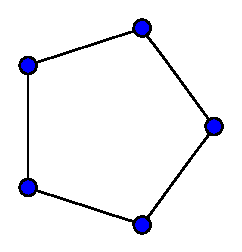
\includegraphics[width=0.25\textwidth]{pentagon.eps}
  \caption{The Pentagon}
  \label{fig:pentagon}
\end{figure}

\begin{remark}[Notation]
  Let $G$ be a graph.

  % reword access, ensure that these accessors are useful
  \begin{itemize}
  \item Let $G = (V,E)$ be a graph. For convenience, we will use subscript
    notation to refer to the edge and vertex sets of $G$, i.e. $V_G = V$ and
    $E_G = E$.
  \item $v \in G$ is an equivalent statement to $v \in V_G$
  \item $|G|$, called the \textbf{order} of $G$, is equal to $|V_G|$.
  \end{itemize}
\end{remark}

When we speak about graphs, we are concerned with the structure of the graph
rather than the specific symbols in its vertex set. Thus we use the following
definition of equality.

\begin{definition}[Equivalence of graphs]
  Two graphs $G$ and $H$ are equivalent if there exists a bijection $\phi : V_G \to V_H$
  such that $\{u,v\} \in G$ if and only if $\{\phi(u),\phi(v)\} \in H$.
\end{definition}

Equivalence of graphs induces an equivalence relation on the set of all graphs. For convenience, we
will often only discuss graphs up to this equivalence relation (which only affects vertex labels).

\begin{example}
  \label{ex:basic_graphs}
  The \textbf{empty graph} of order $n$ is the graph such that $|V| = n$ and $E
  = \varnothing$.

  The \textbf{complete graph} of order $n$, denoted $K_n$, is the graph containing every possible
  edge, so that $|E_{K_n}| = \frac{n(n-1)}{2}$.

  We say a graph is \textbf{bipartite} when there exists a bipartition of its vertex set such that
  there are no edges between vertices in the same part. The \textbf{complete bipartite graph},
  denoted $K_{n,m}$, is such a graph where the two partitions have cardinality $n$ and $m$
  respectively, and every pair of vertices in distinct partitions is joined by an edge.
\end{example}

\begin{figure}[H]
  \centering
  
\includegraphics[width=0.4\textwidth]{k34.eps}
  \caption{The complete bipartite graph $K_{3,4}$}
  \label{fig:k34}
\end{figure}

\begin{definition}
  The \textbf{neighborhood} of a vertex $u \in G$, denoted $N(u)$, is the set of all vertices $v$
  such that $\{u,v\} \in E_G$, and these $v$ are called the neighbors of $u$. The \textbf{degree} of
  $u$ is defined by $\deg(u) = |N(u)|$. A graph in which every vertex has the same degree is
  \textbf{regular}. If that degree is equal to $k$, then the graph is said to be $k$-\textbf{regular}.
\end{definition}

\begin{example}
  $K_n$ is an $(n-1)$-regular graph, $K_{n,n}$ is an $n$-regular graph, and the pentagon is a
  $2$-regular graph.
\end{example}

\begin{definition}
  \label{def:walk_path}

  A \textbf{walk} of a graph $G$ is an alternating sequence of edges and vertices such that each
  vertex is incident to the edges before and after it.

  A \textbf{path} is the sequence of edges in a walk where every vertex is unique.

  The \textbf{shortest-path distance} between two vertices $u,v \in G$, denoted $\spd(u,v)$, is the
  minimum number of edges in a path from $u$ to $v$.
\end{definition}

\begin{definition}
  \label{def:adj_mat}
  The \textbf{adjacency matrix} $A$ of a graph $G$ is given by
  \[
    A_{ij} = \begin{cases}
      1 &: \{v_i,v_j\} ~\text{is an edge in $G$} \\
      0 &: \text{otherwise} \\
    \end{cases}
  \]

  where the set $\{v_i\}_{i=1}^{|G|}$ is an ordering of the vertices in $G$.
\end{definition}
 
%% Adjacency matrix properties
% - symmetric, (eigenvalues are real)
% - eigenvectors
% - spectral gap (+ defn)
% - example: k-regular graphs have largest (simple?) eigenvalue

Note that the adjacency matrix of a graph is not unique in general. Depending on
the way that the vertices of $G$ are numbered, we may end up with a different
matrix. However, for every adjacency matrix the following holds:


\begin{definition}
  A matrix is \textbf{reducible} if and only if it can be put in block upper triangular
  form by simultaneous row and column permutations. In other words, a matrix $M$
  is reducible if and only if there exists a permutation matrix $P$ such that
  $P^{-1}MP$ is block upper triangular. Otherwise, it is said to be
  \textbf{irreducible}.
\end{definition}

\begin{proposition}
  \label{prop:adj}
  Let $A$ be the adjacency matrix of a graph $G$. Then the following are true:

  \begin{enumerate}
  \item $A$ is symmetric (so the eigenvalues of $A$ are real)
  \item $A$ corresponds to a graph that is unique up to equivalence
  \item $A$ is irreducible if and only if $G$ is connected
  \end{enumerate}
\end{proposition}

\begin{proof}
  We omit proofs for (1) and (2) as they are self-evident.

  For (3), we first observe that $P^{-1}AP$ is an adjacency matrix of a graph
  equivalent to $G$ for any permutation matrix $P$. So without loss of generality, suppose that $G$ is
  connected and $A$ is already in block upper triangular form. Then because $A$
  is symmetric, we have

  \[
    A = \begin{bmatrix}
      B & \mathbf{0} \\
      \mathbf{0} & C
    \end{bmatrix}
  \]

  where $B$, $C$, are square block matrices. Say that $B$ has size $m \times m$. It is clear that
  there are no edges connecting the vertices in $\{1, ..., m\}$ to those in $\{m+1, ..., n\}$. Thus
  $G$ is not connected, which is a contradiction.
\end{proof}

The irreducibility result allows us to apply the Perron-Frobenius Theorem, resulting immediately in
these additional properties of $A$.

\begin{theorem}[Pg 673 (section 8.3) of ~\cite{alma991790573504746}]
  \label{thm:perron_frobenius}
  Let $A$ be an irreducible nonnegative square matrix of order $n$. The
  following is true.

  \begin{enumerate}
  \item Let $r$ be the maximum magnitude of the eigenvalues of $A$. Then $r$ is
    a (real, positive) simple eigenvalue of $A$.
  \item The eigenvalue $r$ has left and right eigenvectors whose components are
    all positive
  \item The only eigenvectors of $A$ whose components are all positive have
    eigenvalue $r$.
  \item
    \[ \min_i \sum_j a_{ij} \leq r \leq \max_i \sum_j a_{ij} \]
  \end{enumerate}
\end{theorem}

Because $A$ is nonnegative and irreducible for all connected graphs, these
properties hold for all such adjacency matrices. Indeed, the irreducibility and
nonnegativity of $A$ yields many other interesting properties which we omit
here.

\begin{definition}
  The \textbf{spectral gap} of a matrix $A$ is $\max_{i,j}|\lambda_i - \lambda_j|$, where
  $\lambda_i$ and $\lambda_j$ are the two largest eigenvalues of $G$.

  The \textbf{spectral gap of a graph} is the spectral gap of its adjacency matrix.
\end{definition}

We will next explore graph Laplacians, whose spectra are closely related to
those of adjacency matrices.

\begin{definition}
  \label{def:deg_mat}
  The \textbf{degree matrix} of $G$ is the diagonal matrix defined by
  \[
    D_{ij} = \begin{cases}
      \deg(i) &: i = j \\
      0 &: i \neq j
    \end{cases}
  \]
\end{definition}

\begin{definition}
  The \textbf{graph laplacian} of $G$ is given by $L = D - A$, where $D$ is the
  degree matrix of $G$ and $A$ is the adjacency matrix. In other words,

  \[
    L_{ij} = \begin{cases}
      \deg(i) &: i=j \\
      -1 &: (i,j) ~\text{is an edge in $G$} \\
      0 &: \text{otherwise}
    \end{cases}
  \]
\end{definition}

\begin{proposition}
  %%%%% \begin{enumerate}
  %%%%%   \item 
  %%%%% \end{enumerate}
  Let $G$ be a $k$-regular graph, $\{\lambda_i\}$ and $\{x_i\}$ be the sets of eigenvalues and
  eigenvectors for its adjacency matrix $A$, and $L$ be the graph Laplacian of $G$. Then
  \begin{enumerate}
  \item $\{\lambda_i - k\}$ is the eigenvalue set of $L$, and
  \item $\{x_i\}$ is the eigenvector set of $L$
  \item $L$ and $A$ have the same spectral gap
  \end{enumerate}
\end{proposition}

\begin{proof}
  Because $G$ is regular, the degree matrix $D$ is equal to $kI$. Let ant $x_i$ be given. Then
  \begin{align*}
    Lx_i &= (A-D)x_i \\
         &= \lambda_ix_i - kx_i \\
         &= (\lambda_i - k)x_i
  \end{align*}

  Which simultaneously shows (1) and (2). (3) follows trivially from (1).
\end{proof}

%% Graph laplacian discussion
% adjacency and eigenvalues relationship

% relationship between graph laplacian eigenvalues & spectracl gap

% eigenvalue distribution of A or L

% Wigner distribution for graph eigenvalues

% see random matrix theory "semicircle law"

% what happens when this is exponential?


\section{Small-World and Scale-free Networks}
\label{sec:small_world}

Small-world networks are a class of graphs characterized by having a very small
average shortest-path distance between any two vertices compared to the overall
size of the graph.

% eigenvalues and eigenvectors

\begin{definition}
  The \textbf{characteristic path length} of a graph $G = (V,E)$ is the average
  distance between vertices in the graph, which is given by

  \[ L_G = \frac{1}{|E|} \sum_{\substack{u,v \in V \\ u \neq v}} \dist(u,v)\]

  where $\dist(u,v)$ is shortest-path distance. 
\end{definition}

\begin{definition}[Page 1 of ~\cite{PhysRevLett.90.058701}]
  Consider a graph $G = (V,E)$. $G$ is a \textbf{small-world network} if
  $L_G \sim \log{|V|}$.
\end{definition}

Small-world networks are ubiquitous in a variety of applications areas. However, many real-world
examples of such graphs also have other distinctive structural properties which are not necessarily
captured by their small-worldedness alone ~\cite{Barabasi509}. Thus, we introduce the following
definition:


% We can partially describe this structure in terms of the
% clustering coefficient.

% \begin{definition}
%   Let $v$ be a vertex in a graph $G = (V,E)$.

%   Consider the subgraph formed by the neighborhood of $v$. This subgraph has at
%   most $\deg(v)(\deg(v) - 1)$ edges, which happens when it is a clique. Denote
%   the number of edges of the neighborhood subgraph by $E_{N(v)}$.

%   The \textbf{clustering coefficient} $C_v$ is defined by
%   $C_v = \frac{E_{N(v)}}{\deg(v)(\deg(v) - 1)}$, that is, $C_v$ is the
%   proportion of edges in the neighborhood subgraph out of all possible edges.
%   The clustering coefficient of $G$ is the average of all vertex clustering
%   coefficients, $C_G = \frac{\sum_{v \in V}{C_v}}{|V|}$.
% \end{definition}

\begin{definition}[Pg. 1 of ~\cite{PhysRevE.71.027103}]
  A \textbf{scale-free network} is a graph whose vertex degrees follow a power
  law. That is, given a randomly selected $u \in G$,
  $P(\deg(u) = k) \sim k^{-\gamma}$ for some $\gamma > 0$.
\end{definition}

One of the defining characteristics of power law distributions is that they have
very long tails. In a scale-free graph with many vertices, this implies the
existence of \textbf{hubs}, which we informally define as vertices whose degrees
are far larger than average in the graph.

Real world examples of scale-free networks are abundant and include the world
wide web, cellular communication networks, and protein-protein interaction (PPI)
networks. It is not surprising, then, that scale-free networks are necessarily
small-world networks, however we defer to Cohen and Havlin for proof of this
fact.

\begin{theorem}[Final result of ~\cite{PhysRevLett.90.058701}]
  Scale-free networks are small-world networks.
\end{theorem}



\section{Random Graphs}
\label{sec:random_graphs}

% exponential distribution eigenvalues

\begin{definition}
  A \textbf{random graph} is a random variable for which all outcomes are
  undirected graphs.

  A \textbf{random graph process}, denoted $(G_t)$, is a family of random graphs
  indexed by a discrete time $t \in \mathbb{N}$.
\end{definition}

We are interested in random graph processes which build small-world networks.
The Watts-Strogatz graphs are an example of such a process. They are defined by
starting with a regular ring lattice and randomly rewiring edges until the graph
is obtained.

\begin{definition}
  An $n$-$k$ \textbf{regular ring lattice} is a graph $(V, E)$ with $n$ vertices
  such that $u,v$ is an edge if and only if $|u-v| \leq \frac{k}{2}$.
\end{definition}

\begin{definition}
  Let $v$ be a vertex in a graph. We can \textbf{rewire} $v$ by deleting one
  edge of $v$ and drawing a new one by sampling uniformly from all vertices that
  do not share an edge with $v$.
\end{definition}

\begin{definition}
  Given a probability $p$ and regular ring lattice parameters $n$ and $k$, we
  define the $(n,k,p)$ \textbf{Watts-Strogatz Process} as follows.

  Let $r(G,v)$ be a random process that rewires vertex $v$ in a graph $G$. We
  define a family of graphs, $(G_t)$, by

  \[
    G_{t+1} = \left\{
      \begin{array}{lc}
        r(G_t,t) &: X \leq p \\
        G_t &: X > p
      \end{array}
    \right.
  \]

  for $t = 1,\dots, |G|$, where $G_0$ is the $n$-$k$ regular ring lattice, and
  $X$ is a uniform random variable in the range $[0,1]$. That is, we iterate
  over the vertices of the ring lattice and rewire each one with probability
  $p$.

  We call graphs sampled from $G_{|n|}$ \textbf{Watts-Strogatz graphs}.
\end{definition}

Watts and Strogatz showed empirically that the Watts-Strogatz graphs are small-world networks for all
but extremely small values of $p$~\cite{Watts1998Collective}. However, in general, they are not scale
free networks~\cite{Barabasi509}, and thus do not show the structural characteristics of many
practical data sets.

% TODO: ask about restated definitions
\begin{definition}[Pg. 511 of ~\cite{Barabasi509}]
  \label{def:ba}
  Let any graph $G_0$ be given as well as some parameter $m$, $m \leq |G_0|$. We
  build the random graph $G_{t+1}$ by adding a new vertex to $G_t$ and
  connecting it to $m$ vertices of $G_t$ with probabilities proportional to the
  degree of each vertex. That is, the probability of adding an edge to a vertex
  $u$ is

  \[
    p_u = \frac{\deg(v)}{\sum_{v \in G_t} \deg(v)}
  \]

  on the first step, and this is done a total of m times without replacement.

  We call $(G_t)$ the $(G_o,m)$-\textbf{Barab\'asi-Albert (BA) process} and graphs
  sampled from $G_n$ $(G_o,m,n)$-\textbf{Barab\'asi-Albert (BA) graphs}.
\end{definition}

This type of model, where edges to a new vertex are drawn with non-uniform
probability, is known as \textbf{preferential attachment}.

\begin{theorem}[Pg. 511 of ~\cite{Barabasi509}]
  \textbf{Barab\'asi-Albert graphs} are scale-free
\end{theorem}

The scale-free-ness of BA graphs makes them an attractive model, as they are likely to have degree
distributions similar to those of many real data sets. In addition, BA graphs are guaranteed to be
connected.

%%% Local Variables:
%%% mode: latex
%%% TeX-master: "../Main"
%%% End:



\chapter{Random Labeled Graphs}
\label{chap:random_graphs}
We wish to use random graphs to test vertex classifiers. An issue that arises is that the generative
models presented so far do not suggest any natural labeling for the vertices of the resultant graphs.
Thus, we propose some models for generating labeled small-world and scale-free networks.

\begin{definition}
  A \textbf{labeled graph} is a graph $G$ and a function $c : V_G \to S$, where $S$ is an arbitrary.
  For $u \in V_G$, we call $c(u)$ the \textbf{class} of $u$.
\end{definition}

In considering labeled graphs, it is useful to look at not only at each vertex's degree, but also the
number of neighbors with the same label vs the number of neighbors with a different label. For
convenience, we define these quantities as follows:

\begin{definition}
  Let $G$ be a labeled graph, $u \in V_G$. The \textbf{same-class degree} of $u$, $\deg_{same}(u)$, is
  the number of vertices in the neighborhood of $u$ in the same class as $u$. Similarly, $\deg_{diff}(u) =
  \deg(u) - \deg_{same}(u)$ is the number of vertices in a different class.
\end{definition}


\section{Noisy Complete Components (NCC) Graphs}

\begin{definition}
  Let $m$ be a natural number. We construct the \textbf{complete components
    graph} of order $n = 2m$ as follows. Let $V = \{1,2, ..., 2m\}$, and then define
  $E$ by

  \[
    E = \{ (u,v) : u,v \in \{1,...,m\} ~\text{or}~ u,v \in \{m+1,...,2m\} \}
  \]

  i.e. the disjoint union of two complete graphs of order $m$. In addition, we label the graph by the
  function

  \[c(u) =
      \begin{cases}
        0 &: u \in \{1,...,m\} \\
        1 &: u \in \{m+1,...,2m\}
      \end{cases}
    \]
\end{definition}

\begin{definition}
  \label{def:ncc}
  Let parameters $(m,p,q)$ be given, $m \in \mathbb{N}$ and $p,q \in [0,1]$, and let $G_0$ be the
  complete components graph of order $2m$. We construct a \textbf{Noisy Complete Components (NCC)}
  graphs as follows.

  Iterate over ever pair of vertices in the graph (i.e. the edge set of
  $K_{2m}$). For every pair $(u,v) \in E_{G_0}$, that is, for the edges that
  already exist in $G_0$, we delete the edge with probability $q$. Likewise, for
  each pair $(u,v) \notin E_{G_0}$, we add the edge $(u,v)$ with probability
  $p$.

  The resultant graph is an NCC graph. We can also observe a natural generalization to graphs with more than two complete components.
\end{definition}

We will now inspect the properties of such graphs in order to demonstrate that they are, in fact,
small worlds graphs in the subset of the parameter space in which we're interested. Before doing so,
we recall some basic distributions from statistics

\begin{definition}
  A \textbf{Bernoulli distribution} with probability $p$ is a discrete probability distribution
  with probability mass function

  \[
    f(x) =
      \begin{cases}
        p &:~ x = 1 \\
        1-p &:~ x = 0 \\
        0 &:~ \text{otherwise}
      \end{cases}
    \]

  A \textbf{binomial distribution} of $n$ trials with probability $p$, denoted $B(n,p)$ is equal to
  the sum of $n$ independent bernoulli random variables with probability $p$. Its probability mass
  function is

  \[
    f(x) = {n \choose x} p^x(1-p)^{n-x}
  \]

  for $x = 0,1,...,n$ and $0$ outside that range.

  For a more complete discussion of these distributions and the probabilitity theory employed in
  this chapter, see ~\cite{CaseBerg:01}.
\end{definition}


\begin{theorem}
  \label{thm:ncc_deg}
  Let $G$ be an $(m,p,q)$ NCC graph and $u$ a vertex in $G$. Then $\deg(u)$ follows the distribution
  $X + Y$, where $X$ and $Y$ are (independent) binomial random variables, $X \sim B(m-1,1-q)$ and
  $Y \sim B(m,p)$. Moreover, $\deg_{same}(u) = X$ and $\deg_{diff}(u) = Y$.
\end{theorem}
\begin{proof}
  First, observe that adding and deleting edges to an NCC graph is done independently for each edge.
  In other words, the existence or nonexistence of any edge of $G$ is independent of every other edge.
  In addition, the number of edges added between $u$ and all other different-class vertices is equal
  to a sum of $m$ Bernoulli random variables of probability $p$, because there are $m$ possible edges
  from $u$ to the opposite class. Thus $deg_{diff}(u)$ follows a binomial distribution on $m$ trials,
  $deg_{diff}(u) = Y \sim B(m,p)$.

  In the case of same-class edges, we will consider the probability that an edge is \textit{preserved}
  rather than deleted. Edges are preserved with probability $(1-q)$, so as in the different-class
  case, we can see that the same-class degree of $u$ follows a binomial distribution on $(m-1)$
  trials, $deg_{same} = X \sim B(m-1,1-q)$.

  As we've counted both the same- and different-class degrees, it is clear that $deg(u) = X + Y$.
\end{proof}

We must take care to note that this is not the same thing as the degree distribution over the whole
graph $G$. While each edge with respect to a single vertex is picked independently, this is not true
over the whole graph, since each edge is connected to two vertices.

\begin{remark}
  The previous theorem shows that the following is true
  \begin{enumerate}
  \item $\E(\deg_{same}(u)) = (m-1)(1-q)$ and $\E(\deg_{diff}(u)) = mp$, where $\E$ is expectation.
  \item $\Var(\deg_{same}(u)) = (m-1)(1-q)q$ and $\Var(\deg_{diff}(u)) = mp(1-p)$, where $\Var$ is
    variance.
  \item $\E(\deg(u)) = (m-1)(1-q) + mp$ by linearity of expectation.
  \item $\Var(\deg(u)) = (m-1)(1-q)q + mp(1-p)$ by linearity of variance on independent random
    variables.
  \end{enumerate}
\end{remark}

% \begin{theorem}
%   Let $u$ and $v$ be vertices in an $(m,p,q)$ NCC graph. We write $P(\spd(u,v) = k)$ for the probability
%   that the shortest path between $u$ and $v$ is equal to $k$.

%   If $c(u) = c(v)$, then $\E(P(\spd(u,v) = 1)) = 1-q$ and
%   $\E(P(\spd(u,v) = 2)) = 1- (1 - (1-q)^2)^{m-1} (1-p^2)^{m}$.

%   If $c(u) \neq c(v)$, then $\E(P(\spd(u,v) = 1)) = mp$ and
%   $\E(P(\spd(u,v) = 2)) = 1- ((1-q)(1-p) + q)^{m-1}(pq+(1-p))^n$.
% \end{theorem}
% \begin{proof}
%   For the cases where $\spd(u,v) = 1$, the results follow immediately from definition \ref{def:ncc}.

%   \textbf{Note to Professors:} while typing this, I found an error. I need to nudge around the random
%   variables in the probability formulas because I'm operating under the assumption that 1) there's an
%   edge between $u$ and each neighbor, and 2) there's not an edge between $u$ and $v$. This just
%   reduces the number of trials on the binomial variables so it should just be changes by factors of $p$
%   and $q$, but I didn't have time to work it out.

%   % TODO: fix this. X changes slightly because we assume that the trial between u and v failed, and
%   % the trial between u and each neighbor succeeded.
%   Now, we consider the case where $\spd(u,v) = 2$ and $c(u) = c(v)$. Under these circumstances, we
%   denote the number of same-class neighbors by the random variable $X$ and the number of
%   different-class neighbors by $Y$. A length-2 path between $u$ and $v$ must exist unless we fail to
%   preserve/add every single edge from the neighborhood of $u$ to $v$, which happens with probability
%   $q^X(1-p)^Y$. Thus $P(\spd(u,v) = 2) = 1 - q^X(1-p)^Y$.

%   Since $X$ and $Y$ are binomial random variables by theorem \ref{thm:ncc_deg}, their probability mass
%   functions are:

%   \begin{align*}
%     f_X(x) &= {n-1 \choose x} (1-q)^xq^{n-1-x} \\
%     f_Y(y) &= {n \choose y} p^y(1-p)^{n-y}
%   \end{align*}

%   using the expectation formula, we can compute $q^x$ and $p^Y$:

%   \begin{align*}
%     \E(q^X) &= \sum_{i=0}^{n-1}q^i{n-1 \choose i}(1-q)^iq^{n-1-i} \\
%             &= q^{n-1}\sum_{i=0}^{n-1}{n-1 \choose i}(1-q)^i(1)^{n-1-i} \\
%             &= q^{n-1}(2-q)^{n-1} \\
%             &= (1 - (1 - q)^2)^{n-1}
%   \end{align*}

%   \begin{align*}
%     \E((1-p)^Y) &= \sum_{i=0}^{n}(1-p)^i{n \choose i}(1-(1-p))^i(1-p)^{n-i} \\
%             &= (1-p)^{n}\sum_{i=0}^{n}{n \choose i}(1-(1-p))^i(1)^{n-i} \\
%             &= (1-p)^{n}(p-1))^{n} \\
%             &= (1 - p^2)^{n}
%   \end{align*}
%   thus, in this case,

%   \[ P(\spd(u,v) = 2) = 1 - (1 - (1-q)^2)^{n-1}(1-p^2)^n \]

%   % TODO: fix this. Y changes slightly because we assume that the trial between u and v failed.
%   In the case where $c(u) \neq c(v)$, the probability becomes $P(\spd(u,v) = 2) = 1 - q^Y(1-p)^X$, so
%   by an analogous computation, we get

%   \[ P(\spd(u,v) = 2) = 1 - (q + (1-p)(1-q))^{n-1}(pq + (1-p))^n \]
% \end{proof}


These graphs are extremely regular, so they do not exhibit scale-free properties. Thus, we
also propose a variant on the Barab\'asi-Albert model which adds labels while preserving the power
law degree distribution.

%% prove theorem: the following are equal: frobenius norm of a matrix,
%% \sum{\lambda^2}, number of edges in G (or something like this)

% sketch: recall \sum \lambda_i = \tr(M). Consider A^2, whose trace is the sum
% of degrees

\section{Class-Weighted Barab\'{a}si-Albert (CWBA) Graphs}

% TODO: refer back to previous chapter definition of BA 
\begin{definition}
  Let parameters $G_0$ and $m \leq |G_0|$ be given as in the BA process as well
  as a finite set of labels $S$ and a factor $\rho \ge 1$. In addition, suppose
  each vertex in $G_0$ has been labeled by an element of $S$. Given a graph
  $G_t$, we build $G_{t+1}$ as follows.

  As in the BA process (see definition \ref{def:ba}, page \pageref{def:ba}), we will add one new vertex and draw
  edges using preferential attachment, however, we label our new vertex $l$, which is chosen from $S$
  with uniform probability. Then, we reweight the probability of drawing each edge in order to favor
  vertices with label $l$ by a factor of $\rho$.

  Define $S_l$ to be the set of vertices with label $l$. Then, we define the
  probability of drawing an edge to a vertex $u$ as

  \[
    p_u = \begin{cases}
      \frac{\rho\deg(u)}{w} &: u \in S_l\\
      
      \frac{\deg(u)}{w} &: u \in (V_G - S_l)\\
    \end{cases}
  \]

  where $w$ is the weighted degree sum,

  \[
    w = \rho \sum_{v \in S_l}\deg(v) + \sum_{v \in (V_G - S_l)}\deg(v)
  \]

  We call this random process the \textbf{class-weighted Barab\'asi-Albert
    (CWBA) process} and we call graphs sampled from this model \textbf{CWBA
    graphs}.

  % TODO: add example
\end{definition}

We do not prove that CWBA graphs are scale-free, but degree plots over arbitrary choices of
parameters suggest that they are. See figure ~\ref{fig:cwba_degs}.

\begin{figure}[H]
  \centering
  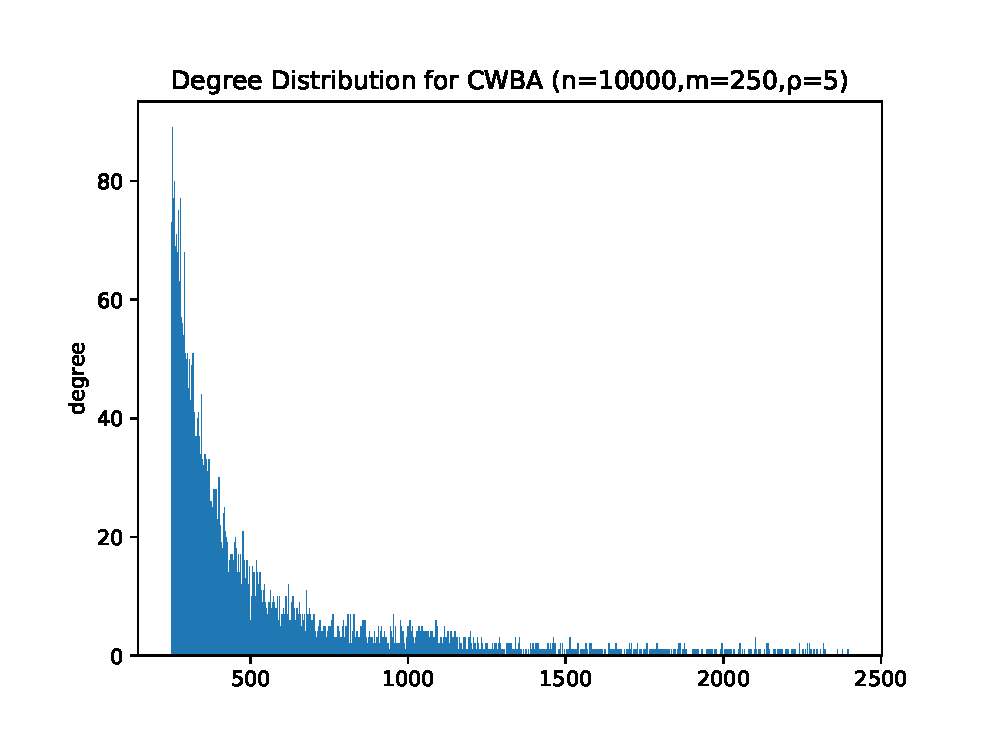
\includegraphics[width=0.7\textwidth]{CWBA_degree_dist.eps}
  \caption{Degree distribution of CWBA graphs demonstrates clear scale-free behavior.}
  \label{fig:cwba_degs}
\end{figure}

Between the apparent power law degree distribution and the straightforward reweighting of the
preferential attachment algorithm, we expect CWBA graphs to be a reasonably good indicator of how a
metric-based classifier would perform on real-world data.

%%% Local Variables:
%%% mode: latex
%%% TeX-master: "../Main"
%%% End:


\chapter{Metrics on Graphs}
\label{chap:metrics}
In this chapter, we provide background about metrics on graph vertices, with a particular focus on
the diffusion state distance (DSD). The three prediction algorithms compared in Chapters
\ref{chap:simulations} and \ref{chap:real_world} are identical except for the choice of metric, as a
key part of our project is understanding how that choice affects label prediction performance. For
details about how our classification algorithm uses metrics to pick labels, see Chapter
\ref{chap:prediction}.


\section{Definition and Shortest-Path Distance}

A metric is a nonnegative real-valued function that generalizes Euclidean distance between points in
$\mathbb{R}^n$ to general sets. In our case, the set is the vertices of the graph, and in the context of the
label prediction problem, we use metrics to determine similiarity of two vertices in the graph.

\begin{definition}
  A \textbf{metric} on a set $S$ is a function $f : S \times S \to \R$
  satisfying

  \begin{enumerate}
  \item $f(u,v)\geq 0 ~ \forall u,v \in G$,
  \item $f(u,v) = 0 \iff u = v$ (identity of indiscernables),
  \item $f(u,v) = f(v,u) ~\forall u,v \in G$, and
  \item $f(u,v) \leq f(u,w) + f(v,w) ~\forall u,v,w \in G$
    (triangle inequality).
  \end{enumerate}
\end{definition}

The standard metric on graphs is the shortest-path distance (definition \ref{def:walk_path}), whose
definition we reiterate here for convenience. The \textbf{shortest-path distance} between two
vertices $u,v \in G$, denoted $\spd(u,v)$, is the minimum number of edges in a path from $u$ to $v$.

\begin{proposition}
  Shortest-path distance is a metric (on the vertices of connected graphs).
\end{proposition}

\begin{proof}
  From the definition of shortest-path distance, it is clear that metric conditions (1), (2),
  and (3) are satisfied, since we're dealing with unweighted, undirected graphs.

  To prove (4), let any three vertices in a connected graph $u,v,w$ be given. Define $a=\spd(u,w)$
  and $b=\spd(v,w)$. Then there exists a path from $u$ to $w$ of length $a$ and from $w$ to $v$ of
  length $b$, and concatenating these paths gives a path from $u$ to $v$ of length $a+b$. Thus, by
  definition of shortest-path distance, $\spd(u,v) \leq a + b = \spd(u,w) + \spd(v,w)$ for any three
  vertices $u,v,w$, which is more than sufficient to show (4).
\end{proof}

\section{Resistance Distance}

\begin{definition}[from ~\cite{weissteinRD}]
  Let $G$ be a connected graph. Imagine that $G$ is an electrical network where every edge is a
  1-ohm resistor. The resistance distance between $u,v \in G$, denoted $\rd(u,v)$, is the reciprocal
  of the resistance between $u$ and $v$ as calculated by Kirchoff's laws, with the unit (ohms)
  dropped.

  Formally, we can define it as follows. Let $L$ be the graph laplacian of $G$ and define $\Gamma$
  as

  \[ \Gamma = L + \frac{\mathbf{1}}{n} \]

  where $\mathbf{1}$ is the matrix consisting of all $1$s. Then,

  \[ \rd(u,v) = (\Gamma)^{-1}_{ii} + (\Gamma)^{-1}_{jj} - 2(\Gamma)^{-1}_{ij}\]
\end{definition}

\begin{theorem}[Page 89, Theorem B of ~\cite{KleinRandic1993}]
  $\rd$ is a metric (on the vertices of an arbitrary connected graph)
\end{theorem}

Resistance distance is another example of a metric on graphs, and it is dramatically different from
shortest-path distance. One of its key characteristics is that as we add more paths connecting two
vertices, the distance between them decreases ~\cite{KleinRandic1993}. Because resistance distance
gives consideration to the entire graph (as opposed to just the shortest path), we expect it to be
more stable to noise in the form of randomly added or deleted edges than shortest path.


\section{Diffusion State Distance}

The diffusion state distance (DSD) is a metric on graphs which determines distance between two
vertices based upon the convergence behavior of random walks starting from each vertex. Intuitively,
it provides a way to measure vertex distance that is sensitive to the local structure of the graph,
and appears to be well suited to detecting community structures in graphs.

In the original paper, Cao, Zhang, Park, Daniels, Crovella, Cowen, and Hescott define DSD in terms
of a vector-valued function $\mathrm{He}^{k}(u)$, which computes the expected number of times a
length-$k$ random walk originating at a vertex $u$ will visit each other vertex in the graph. They
compute DSD by taking the $l_1$-norm of the difference between two such vectors in the limit as
$k \to \infty$. We present an alternative definition which is easier to manipulate with the usual
machinery of linear algebra. We begin by recalling some definitions.

\begin{definition}
  A \textbf{random walk} of a graph is a walk (see definition \ref{def:walk_path}) originating at
  some vertex in which each edge is picked uniformly randomly from all the edges adjoined to the
  vertex preceding it.
\end{definition}

\begin{definition}[Page 302 of \cite{Bollobas1998} ]
  A (discrete-time) \textbf{markov chain} on a finite set of states $V$ is a sequence of random
  variables $X_0,X_1,....$ taking values $x_o,x_1,... \in V$ such that for a given $t$, the
  probability of each outcome of $X_{t+1}$ depends only on $x_t$ (the outcome before it).

  Let $u,v \in V$. Then the conditional probability $P(X_{t+1}=v|X_t=u)$ is called the
  \textbf{transition probability} from $u$ to $v$.
  
  The \textbf{transition matrix} of a markov chain is the matrix $T$ given by

  \[
    T_{ij} = \text{The probability of transitioning from state $j$ to state $i$}
  \]
\end{definition}

Random walks may be modeled as markov chains where the states are the vertices in the graph. The
random walk transition matrix of a graph $G$ can be written $T = AD^{-1}$, where $A$ is the
adjacency and $D$ is the degree matrix, (definitions \ref{def:adj_mat} and \ref{def:deg_mat}). For
our purposes, we assume that vertices are labeled by the positive integers $1,2,...,n$ and that the
rows and columns of $G$ correspond to this ordering.

\begin{proposition}[Properties of $T$]
  Let $G$ be a graph and $T$ the transition matrix for the corresponding random walk markov chain.
  The following is true:
  \begin{enumerate}
  \item $T$ is irreducible
  \item every eigenvalue of $T$ has magnitude $\leq 1$
  \end{enumerate}
\end{proposition}

\begin{proof}
  To show (1), we first recall from proposition \ref{prop:adj} that the adjacency matrix is
  irreducible. From the definition $T = AD^{-1}$, we can see that $T$ has zeros in the same set of
  indices as $A$, and so must be irreducible by analogous argument.

  (2) follows from (1) and application of the Perron-Frobenius Theorem (Theorem
  \ref{thm:perron_frobenius}).
\end{proof}

Based on how we've defined the transition matrix, it can be thought of as an operator which takes a
marginal distribution of states in the markov chain, and outputs the marginal distribution after one
step. So, the marginal distribution of vertices in the $k\nth$ step of a random walk originating
from vertex $u$ is given by $T^ke_u$, where $e_u$ is the $u\nth$ standard basis vector in $\R^n$,
$e_{u,u} := 1$ and $e_{u,j} := 0, u \neq j$ for $u=1,...,n$.

Finally, we can define DSD.

\begin{definition}
  Let $G$ be a graph, $u,v \in G$. The \textbf{diffusion state distance (DSD)}, denoted $\dsd(u,v)$,
  is defined by
  \[
    \dsd(u,v) = ||\sum_{k =0}^{\infty}{T^ke_u - T^ke_v}||_1
  \]
  where $T$ is the transition matrix of $G$'s random walk markov chain and $e_i$ is th $i\nth$
  standard basis vector in $\mathbb{R}^n$.
\end{definition}

\begin{theorem}[Page 7 of \cite{10.1371/journal.pone.0076339}]
  DSD is a metric.
\end{theorem}

We defer to Cao et. al for proof of this.

As compared to shortest-path distance, we would expect DSD to be more resilient to random noise in
the form of randomly added and deleted edges. This is because DSD considers the structure of the
entire graph instead of just the shortest path. Resistance distance is also computed using the whole
graph, so we would expect that to be similarly resilient. However, DSD appears to be measuring the
similarity of two vertices' neighborhoods by comparing random walk convergence behavior, whereas
resistance distance is measuring electrical current capacity between two vertices. In the context of
most label prediction problems, where labels correspond to communities, this suggests intuitively
that DSD superior.


\section{DSD on the Complete Graph}

In this section, we work through the problem of computing DSD on the complete graph. This is not a
particularly illuminating result, but we hope it will help to familiarize the reader with the DSD.

Consider the complete graph $K_n$. In this case, $D = (n-1)I$ and $A = (J - I)$, so our transition
matrix $T$ is given by $\frac{1}{n-1}(J-I)$. In order to compute $T^ke_u$ in the limit, we will
represent $e_u$ as a linear combination of eigenvectors of $A$.

\begin{proposition}
  The all-ones vector $1_n$ is an eigenvector of $T$ with eigenvalue $\lambda = 1$, and every
  vector $x \in \R^n$ such that $\sum_i x_i = 0$ is an eigenvector of $T$ with
  $\lambda = -\frac{1}{n-1}$.
\end{proposition}
\begin{proof}
  Multiplying a vector by the all-ones matrix takes the sum of that vector's
  values for every index in the result, so $J \cdot 1_n = n \cdot 1_n$.
  Similarly $Jx = 0_n$, for any $x$ s.t. $\sum_i x_i = 0$. Thus,

  \begin{align*}
    T\cdot 1_n &= \frac{1}{n-1}(J-I) \cdot 1_n \\
               &= \frac{1}{n-1}(n\cdot 1_n - 1_n) \\
               &= 1_n
  \end{align*}

  and

  \begin{align*}
    Tx &= \frac{1}{n-1}(J-I)x \\
       &= \frac{1}{n-1}(0_n - x) \\
       &= -\frac{1}{n-1}x
  \end{align*}
\end{proof}


Next, we will show how to write any $e_u$ as a linear combination of
eigenvectors of $T$. We define $\alpha_u$ by $\alpha_{u,u} := n-1$ and
$\alpha_{u,j} = -1, u\neq j$. The entries of $\alpha_u$ sum to $0$, so
$T\alpha_u=-\frac{1}{n-1}\alpha_u$. We can write
$e_u = \frac{1}{n}(1_n + \alpha_u)$.

\begin{corollary}
  The eigenvectors of $J-I$ span $\mathbb{R}^n$.
\end{corollary}
\begin{proof}
  Since all standard basis elements $e_j$ of $\mathbb{R}^n$ can be expressed as linear
  combinations of eigenvectors for $J-I$, the eigenvectors of $J-I$ span $\mathbb{R}^n$.
\end{proof}

\begin{theorem}
  Let $K_n$ be the complete graph with nodes labelled $1,...,n$. Then for any
  two distinct nodes $u$ and $v$, $\dsd(u,v) = \frac{2(n-1)}{n}$.
\end{theorem}
\begin{proof}
  We will use $\alpha_u$ as defined above. DSD is given by

\begin{align*}
  \dsd(u,v) &= \sum_{k = 0}^{\infty}{||T^ke_u - T^ke_v||_1} \\
              &= \frac{1}{n}\sum_{k = 0}^{\infty}{||T^k(1_n + \alpha_u - 1_n -
                \alpha_v)||_1}\\
              &= \frac{1}{n}\sum_{k = 0}^{\infty}{||T^k(\alpha_u - \alpha_v)||_1} \\
              &= \frac{1}{n}\sum_{k = 0}^{\infty}{||(-\frac{1}{n-1})^k(\alpha_u -
                \alpha_v)||_1} \\
              &= \frac{||\alpha_u - \alpha_v||_1}{n}
                \sum_{k = 0}^{\infty}{(-\frac{1}{n-1})^k} \\
\end{align*}

Since $|-\frac{1}{n-1}| < 1$, the geometric series converges,
$\sum_{k=0}^{\infty}(-\frac{1}{n-1})^k = \frac{n-1}{n}$. When $u \neq v$, the
difference $\alpha_u - \alpha_v$ will have exactly two non-zero entries (since
they are identical at all indices but $u$ and $v$). These non-zero entries will
be $n$ at index $u$ and $-n$ at index $v$. Thus,
$||\alpha(u)-\alpha(v)||_1 = 2n$, and so

\begin{align*}
  \dsd(u,v) &= \frac{2n}{n}(\frac{n-1}{n}) \\
              &= \frac{2(n-1)}{n} \\
\end{align*}

\end{proof}


%%% Local Variables:
%%% mode: latex
%%% TeX-master: "../Main"
%%% End:



\chapter{Label Prediction Methods on Graphs}
\label{chap:prediction}
In this chapter, we define label prediction methods and show how they can
be applied on graphs. We present different problems we can solve using
label prediction methods and how we can incorporate graph metrics, such as
the diffusion state distance (DSD), into these methods. We use the terms
label prediction methods and vertex classifiers interchangeably.

\section{Problem Definition}
\label{sec:label_prediction_methods}
We begin by presenting definitions relating to labels of graphs.

\begin{definition}
A \textbf{partially labeled graph} is a graph $G$ and a function
$c : V_{G_p} \to S$, where $S$ is an arbitrary set of labels, and
$V_{G_p} \subseteq V_G$ with
$|V_{G_p}| = \left\lfloor{p \cdot |V_G|}\right\rfloor$, $0 \leq p \leq 1$.

The set $V_G \setminus V_{G_p}$ is called the set of \textbf{unlabeled} 
vertices of $G$.

The function $c$ is called a \textbf{partial labeling} of $G$.
\end{definition}

\begin{definition}
A \textbf{censoring} of a labeled graph $G$ and its labeling function
$c : V_G \to S$ is a set $V_{G_c}$ and a function
$c_p: V_G \setminus V_{G_c} \to S$ such that $c_p$ is a partial labeling
of $G$.

The function $c$ of the labeled graph $G$ is called the \textbf{ground truth labeling} of the
censoring of $G$. Note that the set $V_{G_c}$ is the set of unlabeled vertices of the partial
labeling of $G$.
\end{definition}

Given a partially labeled graph $G$, a censoring $(V_{G_c}, c_{censor})$
of $G$, and a ground truth labeling $c_{gt}$ of $G$, a 
\textbf{label prediction method} is an algorithm that attempts to correctly 
guess the labels of the unlabeled vertices $V_{G_c}$ with respect to the
ground truth labels $c_{gt}(v), v \in V_{G_c}$.

In order for a label prediction method on a graph to have any success, the ground truth labeling
must reflect some underlying graph structure. If the labels in a graph were assigned at random to
each vertex, a label prediction algorithm could not be expected to perform better than randomly
guessing the labels on vertices.

We now discuss label prediction methods that we considered for our 
simulations in Chapter 6.

% Fix wording make more mathematical
\subsection{Majority Voting Algorithm}
Cao, Zhang, Park, Daniels, Crovella, Cowen, and Hescott~\cite{10.1371/journal.pone.0076339}
describe a simple prediction method called the neighborhood majority voting
algorithm. This algorithm considers each vertex with unknown label and has
its neighbors vote on the label for the vertex. We considered two
implementations of this algorithm, which differ in how they determine which neighbors vote. One 
implementation considers each vertex $v \in V$ and all neighbors of $v$ within an $\varepsilon$
distance from $v$ (a ball of radius $\varepsilon$). The $\varepsilon$ distance depends on the metric
under consideration, and may be changed as a parameter. In an unweighted scheme, each neighbor
within the ball of radius $\varepsilon$ votes equally for their own label. In 
a weighted scheme, we must consider a metric on a graph to use (chapter 4).
Using this metric, each neighbor gets a vote proportional to the reciprocal 
of its distance to the vertex $v$ in
consideration. The other implementation of this algorithm considers each vertex $v \in V$ and
the $k$-nearest neighbors of $v$ with respect to the graph metric. Voting is done similarly in both an unweighted and weighted
scheme.

There are other prediction methods that exist, such as the $\chi^{2}$ neighborhood algorithm, the
multi-way cut algorithm, and the functional flow algorithm~\cite{10.1371/journal.pone.0076339}.
These prediction methods can also be modified to incorporate graph metrics discussed in chapter 4.
However, we only consider the weighted majority voting algorithm for our simulations in order to
keep the intuition behind results of this algorithm simple.

\section{Real World Data}

In this section, we discuss three different examples of graph-based studies performed on real world
data. We discuss how these examples constructed graphs from their data, and what kind of studies
were performed on the resulting graphs. These studies give constructions of different graph
representations of data that we can use to test the effects of different metrics with prediction
algorithms.

\subsection{Protein-Protein Interaction (PPI) networks}
Cao et al.~\cite{10.1371/journal.pone.0076339} studied the prediction of protein
functional labels on the \emph{S. cerevisiae} protein-protein interaction (PPI) network. The
authors constructed a graph using annotated physical interactions in this PPI network. Proteins
corresponded to vertices, and an annotated physical interaction between two proteins corresponded to
an edge. Cao et al. removed redundant edges and the largest connected component was selected,
resulting in a graph of 4990 vertices and 74,310 edges. They also noted that PPI networks are known
to resemble small-world networks, as they have a small maximum shortest path, and a small
characteristic path length. This implies that most vertices in the graph are close to every other
vertex in the graph. One reason for the closeness of vertices in PPI networks was due to hub vertices, which are vertices with very high degree, representing proteins that interact with many other proteins. Figure \ref{fig:PPI_example} shows an example of functional annotation using
the DSD from Cao et al.

\begin{figure}[h] \centering 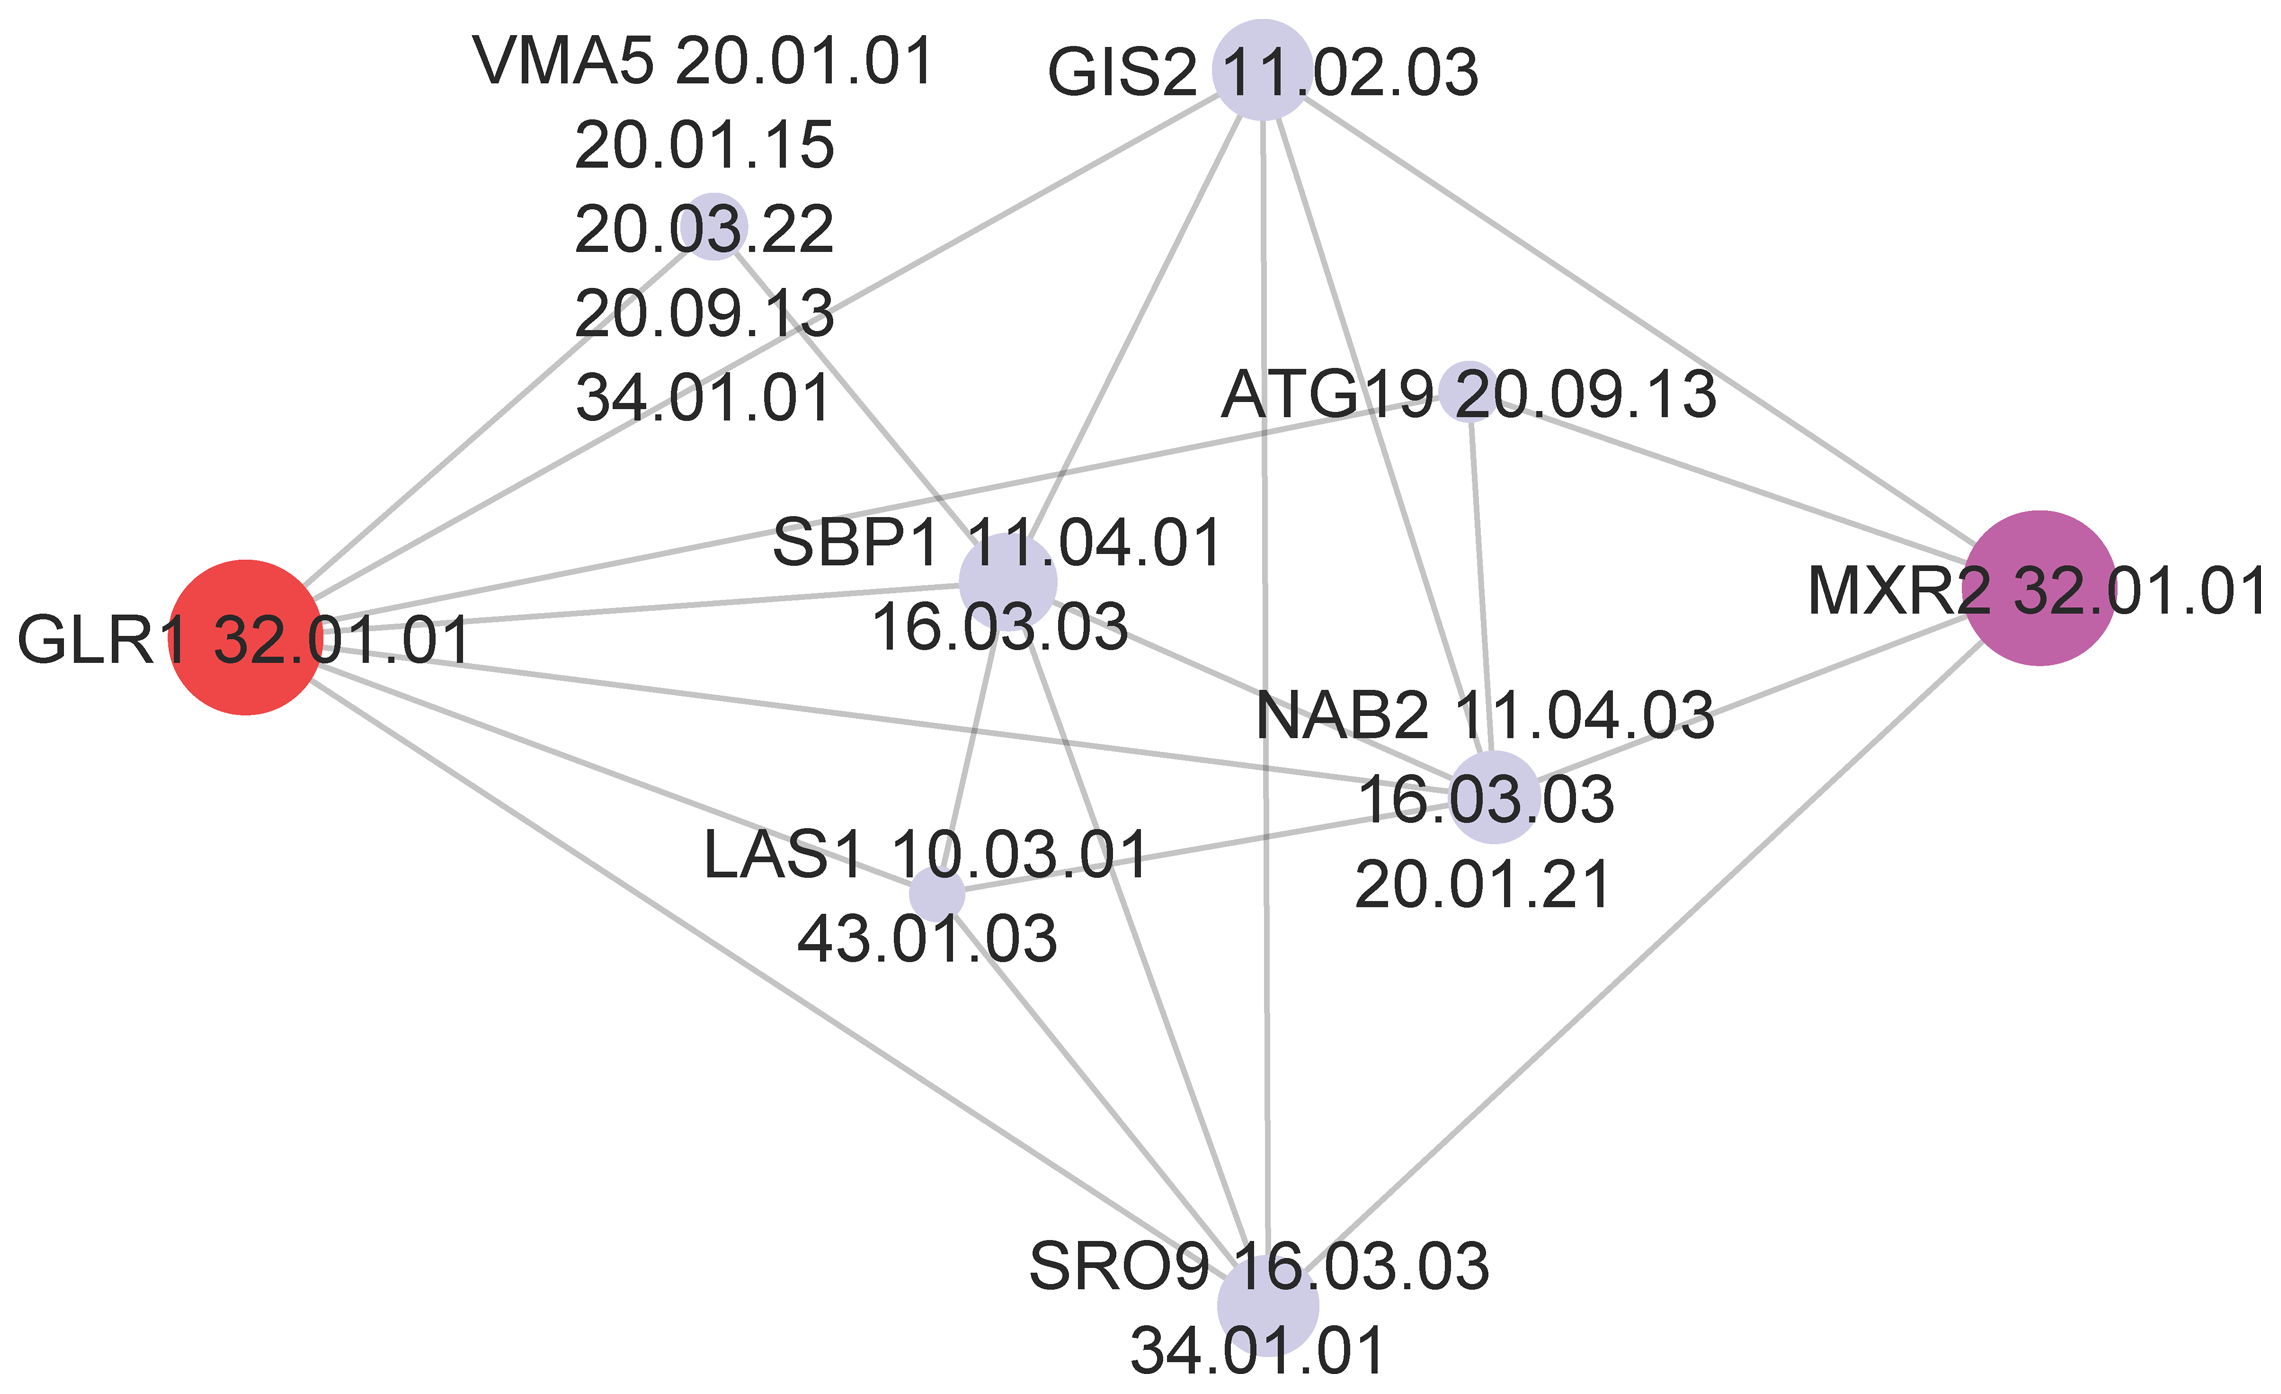
\includegraphics[width=0.75\textwidth]{dsd_ex.png}
\caption{An example of functional annotation with the DSD metric from Cao et al.
~\cite{10.1371/journal.pone.0076339}. It is clear that the vertex colored purple is not a direct
neighbor of the red vertex with respect to the shortest path distance metric. However, the purple
vertex has a DSD distance closest to the red vertex, and they have the same label. Meanwhile, the
direct neighbors of the purple vertex have different labels.}
\label{fig:PPI_example}
\end{figure}

Cao et al. used four different prediction algorithms to compare the effectiveness of the DSD metric
to that of the shortest path metric. Both weighted and unweighted majority voting algorithms, as
well as the $\chi^{2}$ neighborhood algorithm, multi-way cut algorithm, and functional flow
algorithm were used to compare the predictive performance of these metrics. The DSD metric was
expected to perform better that the shortest path metric, since the small characteristic path length
of the PPI network causes the notion of a shortest paths neighborhood to lose significance. All
vertices in this network are close to every other vertex in the graph, so any neighborhood would
contain a large portion of the vertices in the graph.

We used a similar approach in our project, studying the DSD metric and
incorporating it into a label prediction algorithm.

\subsection{Graph model for recommender systems} Huang, Chung, and Chen~\cite{huang2004graph}
introduce a generic graph model for e-commerce transaction data that can support various
recommendation methods. The two-layer graph model proposed represents relationships between products
and customers. In this model, each layer consists of vertices representing products or customers.
Three types of edges in this two layer system capture the inputs to this model from real world data.
Edges between two customers capture similarity based on available demographic data, answers to
questionnaires, and web usage patterns. Edges between two products capture similarity using
descriptions of the product. Finally, edges between customers and products capture transaction
information such as purchase history, customer rating, and related browsing behavior. Figure
\ref{fig:recommender_example} illustrates an example of the two-layer graph model.

\begin{figure}[h] \centering 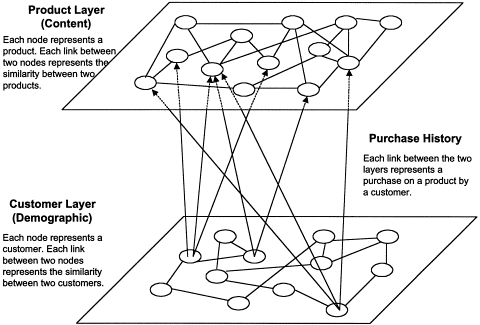
\includegraphics[width=0.75\textwidth]{recommender_ex.png}
\caption{The two-layer graph model proposed by Huang, Chung, and Chen~\cite{huang2004graph}.}
\label{fig:recommender_example}
\end{figure}

Huang, Chung, and Chen considered three different recommendation
methods to use on the model mentioned previously. The direct retrieval method looks at a customer's
previous purchases and products purchased by similar customers to retrieve products to recommend to
the customer. The association mining method uses the purchase history of a customer to generate
association rules about purchasing patterns in order to predict the customer's next purchases. The
high-degree association retrieval method uses weights on edges to represent association strength and
examines paths between the target customer vertex and a product vertex to calculate an association
estimate and determine if the product should be recommended. Transactions from one of the largest
online bookstores in Taiwan were used for data including 9695 books, 2000 customers, and 18,771
transaction records.

The two-layer graph model introduced by Huang, Chung,
and Chen can be interpreted as a graph labeling problem. As a simple example,
we can take the vertices and edges from just the customer layer of the two-layer model. Since the
customer layer included information about demographic data and web usage patterns, we could label
customers with age or certain websites visited and try to predict the labels of prospective
customers. We can perform a similar analysis with the product layer as well as with the whole model
including the interlayer edges.

Such a model can be very useful for advertisers who wish to come up with a
strategic advertising plan. Assuming that an advertisement would have more success if it were shown
to people more likely to buy the product being advertised, we can use the graph model to predict
which customers would buy the product. The product layer can be used to find all products similar to
the product being advertised. Then, we can construct a graph in which vertices are customers who had
bought similar products, and edges existed between customers who had bought the same product.
A prediction algorithm incorporating the DSD could be used to predict the customers who would buy the
product if we knew a few customers that had already bought the product, or were very likely to buy
the product. The DSD proved useful in filtering out hub vertices in the PPI networks, and it may be useful for e-commerce networks as well. Customers with a large amount of purchases may be less informative about product preferences than customers with fewer purchases.

Overall, this study shows that subject-knowledge can be used to create real
world graphs (customer layer, product layer, purchase history). We can extend
this to see how subject-knowledge can be used to determine weights during
the voting process for label prediction methods. Labels can also be 
determined from subject-knowledge. However, these labels must have an
underlying structure or intuition behind them in order for label prediction
algorithms to work.


\subsection{Laplacian Eigenmaps} Belkin and Niyogi~\cite{belkin2002laplacian} propose an algorithm
for constructing a locality-preserving representation of data sampled from a low dimensional
manifold embedded in a higher dimensional space. An example can be found in $n\times n$ gray scale
images of a fixed object taken by a moving camera. These images give data points in
$\mathbb{R}^{n^{2}}$, but the inherent dimensionality of this data should be the number of degrees
of freedom of the camera. The presented algorithm constructs a representation of the data that
reduces the dimensionality of the data.

Belkin and Niyogi construct a weighted graph from a given set of points
in $\mathbb{R}^{n}$. Each point is represented by a vertex, and edges are drawn between neighboring
points. Neighborhoods can be determined using $k$ nearest neighbors or $\varepsilon$-neighborhoods.
Weights are determined using heat kernels, or simply adjacency. Finally, eigenmaps are used to
reduce dimensionality of the data.

$1000$ binary $40 \times 40$ images of vertical and horizontal bars at arbitrary points were
randomly chosen as data. The Laplacian Eigenmap algorithm and Principal Component Analysis (PCA) was
applied to this data and compared. The Laplacian Eigenmap algorithm produced a data representation
that clearly showed separate clusters for the vertical and horizontal bars, which PCA failed to do.

This study is quite different from the previous two studies. However, it still raises some interesting questions and challenges in relation to our project.
The Laplacian Eigenmaps algorithm focused on being able to detect graph structure, assuming that
the given data lies in a lower dimensional manifold. In our project, we try 
to detect properties of graph structure that allow prediction methods
using the DSD to perform well. We could examine whether label prediction
methods using the DSD would be able to detect information about these lower dimensional manifolds.




\chapter{Simulations}
\label{chap:simulations}
In this chapter, we discuss data collected from several simulations run on
our Noisy Complete Components (NCC), Noisy Complete Components with Hubs
(NCCH), and Class-Weighted Barab\'{a}si-Albert (CWBA) models introduced in
Chapter 3. We use these models because they are small-world and have an
intuitive ground truth labeling of vertices. The simple structures of our
models also allow us to test different parameters relating to graph 
structure and examine their effects on prediction accuracies.

For each model, we set a variety of parameters that we want to test.
After constructing the graph, we censor a proportion ($censorP$) of the 
graph, then use a weighted k-nearest neighbors voting (Chapter 5) to solve
a vertex label prediction problem. This process is repeated with the same
parameters $avgRuns$ number of times, and the prediction accuracies
obtained are averaged. We incorporate three different metrics on graphs
(Chapter 4) to our weighted k-nearest neighbors voting algorithm: 
the diffusion state distance (DSD), shortest path distance (SPD), and
resistance distance (RD).


\section{Noisy Complete Components (NCC) Graphs}
% Add more?
In this section, we construct NCC graphs (Chapter 3) and run label 
prediction methods on them.

\subsection{Data Collection}
Our NCC graphs have three input parameters, where $n$ is the number of
vertices in one complete component ($2n$ total vertices), $p$ is the
probability of adding an edge between components, and $q$ is the 
probability of removing an edge within components.

\begin{table}[H]
\centering
\begin{subfigure}[h]{0.4\linewidth}
\begin{tabular}{|l|l|}
\hline
$n$ & $250$ \\ \hline
$p$ & Range from $0$ to $1$\\ \hline
$q$ & $0.5$\\ \hline
$censorP$ & $0.7$\\ \hline
$avgRuns$ & $10$\\ \hline
\end{tabular}
\caption{Fixed $q$}
\end{subfigure}
\hfill
\begin{subfigure}[h]{0.4\linewidth}
\begin{tabular}{|l|l|}
\hline
$n$ & $250$ \\ \hline
$p$ & $0.5$\\ \hline
$q$ & Range from $0$ to $1$\\ \hline
$censorP$ & $0.7$\\ \hline
$avgRuns$ & $10$\\ \hline
\end{tabular}
\caption{Fixed $p$}
\end{subfigure}%
\caption{Tables of parameter values used in our NCC simulations. The table
on the left shows simulation parameters for a fixed $q$, and the table on
the right shows simulation parameters for a fixed $p$.}
\label{table:NCC-params}
\end{table}

Table \ref{table:NCC-params} shows the parameter values we used in our
simulations. The value of parameter $n$ was set to $250$ because this was a
sufficiently large value to allow us to observe differences in prediction
accuracy. Figure \ref{fig:NCC_n} shows that the parameter $n$ only
increases the precision of the prediction accuracies. The parameters $p$
and $q$ were considered probabilities of adding noise to our models, so we
ran simulations to test the effects of these parameters on prediction
accuracies. Figure \ref{fig:NCC_n}(c) shows a plot of the prediction
accuracies over the range of values for $p$, with a fixed $q=0.5$. Figure
\ref{fig:NCC_fixp} shows a plot of the prediction accuracies over the range
of values for $q$, with a fixed $p=0.5$.

\begin{figure}[H]
\begin{subfigure}[h]{0.5\linewidth}
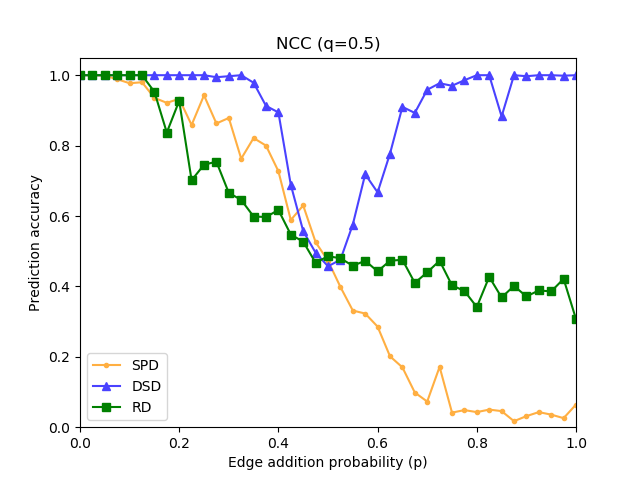
\includegraphics[width=\linewidth]{NCC_fixq_n50.png}
\caption{$n = 50$}
\end{subfigure}
\hfill
\begin{subfigure}[h]{0.5\linewidth}
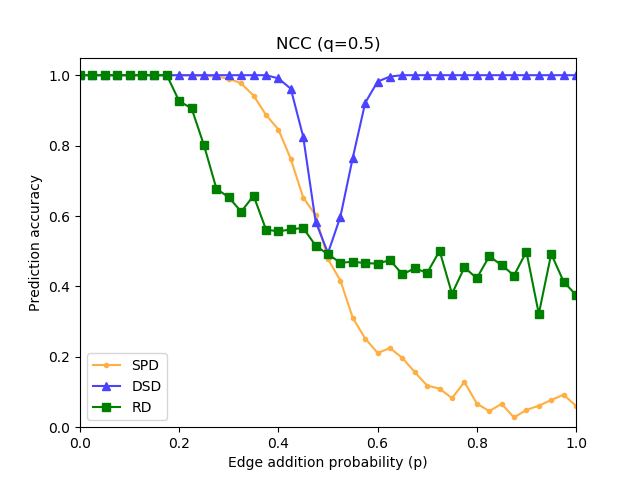
\includegraphics[width=\linewidth]{NCC_fixq_n150.png}
\caption{$n = 150$}
\end{subfigure}
\hfill
\begin{subfigure}[h]{0.5\linewidth}
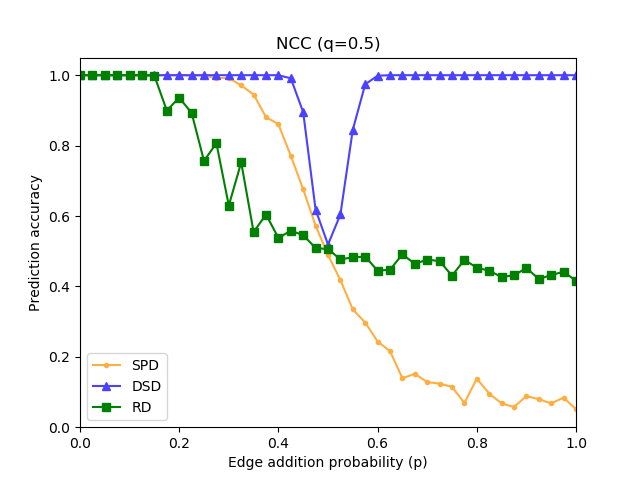
\includegraphics[width=\linewidth]{NCC_fixq_n250.png}
\caption{$n = 250$}
\end{subfigure}
\hfill
\begin{subfigure}[h]{0.5\linewidth}
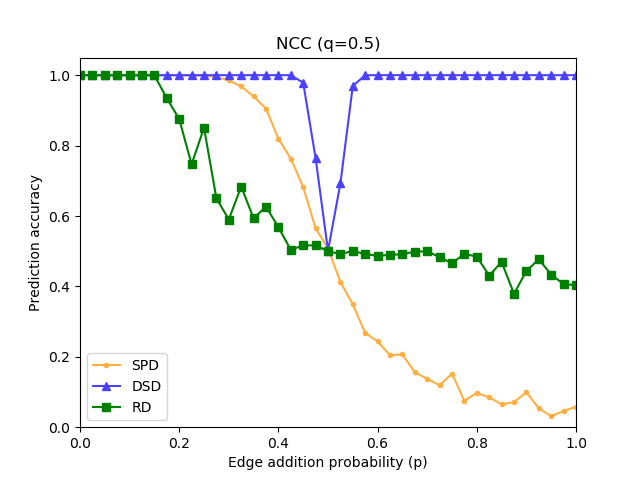
\includegraphics[width=\linewidth]{NCC_fixq_n550.png}
\caption{$n = 550$}
\end{subfigure}%
\caption{These plots show that varying the parameter $n$ in NCC graphs does not change results and a value of $n=250$ will be sufficiently large to observe differences in prediction accuracies. Figure (a) shows that a small value of $n$ may give slightly noisy prediction accuracies due to the smaller number of examples that the prediction accuracies are calculated from.}
\label{fig:NCC_n}
\end{figure}

\begin{figure}[H]
\centering
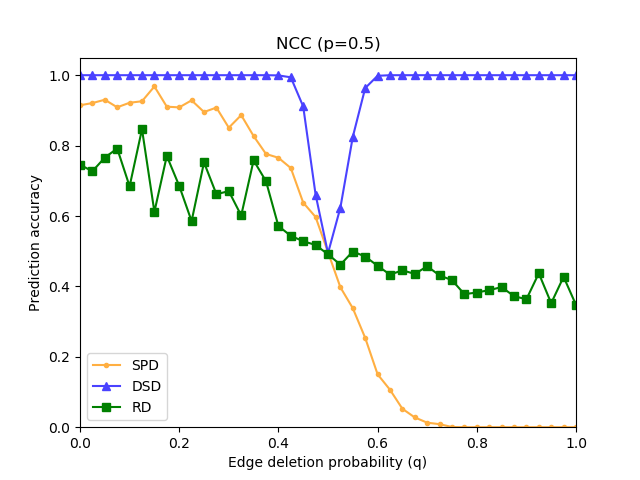
\includegraphics[width=0.8\textwidth]{NCC_fixp.png}
\caption{Plot showing prediction accuracies of the prediction method using the DSD, SPD, and RD metrics. In this simulation, the parameter $p$ was fixed to $0.5$.}
\label{fig:NCC_fixp}
\end{figure}

% Add a part about censorP

\subsection{Analysis}
It is important to note the structure of NCC graphs in extreme cases.
For parameter $p=0$ in NCC graphs (Chapter 3), there is zero probability
of adding edges between components. Since we only consider the largest 
connected component in our analysis, we simply take one of the original components.
If $p=0$ and $q=0$, then we get one complete component. This is not 
interesting, as all prediction methods should attain $100\%$ prediction 
accuracy on these graph. For $p=0$ and $q=1$, we have a set of vertices and no edges. The largest 
connected component would be a single vertex. For $p=1$, there exist edges
from every vertex in one component to every vertex in the other component.
For $p=1$ and $q=1$, we have a complete bipartite graph. We can expect that
a prediction method using the shortest path distance with a small $k$ value
for the $k$-nearest neighbors prediction would result in very poor accuracy
for this method. However, since we have just a binary labeling, these
results can be flipped, making prediction using the inverse of the shortest 
path distance very effective.
With $p=1$ and $q=0$, we have a complete graph where every vertex has equal
same-class degree and different-class degree. This case is not interesting
as all prediction methods would give random results. This leads us to our
next proposition.

\begin{proposition}
For $q = 1 - \frac{mp}{(m-1)}$, NCC graphs are Erd\H{o}s-R\'{e}nyi graphs
with edge probability $p$.
\end{proposition}
\begin{proof}
We know that for NCC graphs (Chapter 3),
$$\E(\deg_{\textit{same}}(u)) = (m-1)(1-q)$$
$$\E(\deg_{\textit{diff}}(u)) = (m)p$$
If $q = 1 - \frac{mp}{(m-1)}$, then we get
$$\E(\deg_{\textit{same}}(u)) = (m-1)(1 - (1 - \frac{mp}{(m-1)})) = mp$$
$$\E(\deg_{\textit{diff}}(u)) = (m)p$$
Thus, we get
$$\E(\deg_{\textit{same}}(u)) = \E(\deg_{\textit{diff}}(u))$$
\end{proof}

The NCC graph with parameters $p$, and $q = 1 - \frac{mp}{(m-1)}$ is expected
to be close to an $(2mp)$-regular graph, where each vertex is expected to 
have the same number of same-class neighbors as different-class neighbors.

The expected number of same-class and different-class neighbors of a vertex
$u$ in an NCC graph corresponds to the expected same-class and 
different-class degrees from Chapter 3. So, from Theorem \ref{thm:ncc_deg}, 
we derive the following result.

\begin{proposition}
For two vertices $u,v$ in an NCC graph,
\begin{enumerate}[(1)]
\item If $u,v$ belong to the same class, they are expected to have 
$$(m-2)(1-q)^2$$ 
common same-class neighbors, and 
$$(m)p^2$$
common different-class neighbors.

\item If $u,v$ belong to different classes, they are expected to have 
$$(2m-2)(1-q)p$$
common neighbors.
\end{enumerate}
\end{proposition}

\begin{proof}
(1) We can see that if $u,v$ belong to the same class, there are $(m-2)$ 
possible same-class vertices that could be common neighbors between them. 
Each of these vertices has a $(1-q)$ probability of being a same-class 
neighbor of $u$ and a $(1-q)$ probability of being a same-class neighbor of 
$v$ (chapter 3). Therefore, we get that the expected number of common same-
class neighbors is $(m-2)(1-q)^2$.

Also, there are $m$ possible different-class vertices that could be common
neighbors between $u$ and $v$. Each of these vertices has a $p$ probability
of being a different-class neighbor of $u$ and a $p$ probability of being a
different-class neighbor of $v$. Therefore, we get that the expected number
of common different-class neighbors is $(m)p^2$.\\

\noindent
(2) If $u,v$ belong to different classes, there are $(2m-2)$ possible 
vertices that could be common neighbors of $u$ and $v$. Without loss of 
generality, each vertex has a $(1-q)$ probability of being a neighbor of $u$
and a $p$ probability of being a neighbor of $v$. Therefore, we get that the
expected number of common neighbors is $(2m-2)(1-q)p$.
\end{proof}

Figure \ref{fig:NCC_n}(c) shows that with a fixed probability of deleting
edges within components of NCC graphs, and a range of probabilities of
adding edges between components of NCC graphs, the label prediction method
using the DSD outperforms the method using SPD and the method using RD.
We can use expected values of same-class degrees (Chapter 3) to reason why
such behavior occurs.

For a fixed $q=0.5$, we can say for any vertex $u$,
$$\E(\deg_{\textit{same}}(u)) = (249)(0.5)$$
$$\E(\deg_{\textit{diff}}(u)) = (250)p$$
We can clearly see that for $p=0.5$, the resulting graph will be random,
having roughly the same number of same-class neighbors as different-class 
neighbors. This explains the near random prediction accuracies when $p$ is
close to $0.5$. However, for $p < 0.5$, we can expect that
$\E(\deg_{\textit{same}}(u)) > \E(\deg_{\textit{diff}}(u))$.
In this case, the prediction method using SPD should predict with high
accuracy, with a sharp decline as the value of $p$ approaches $0.5$. For 
$p > 0.5$, the prediction method using SPD should predict with low 
accuracy, since $\E(\deg_{\textit{same}}(u)) < \E(\deg_{\textit{diff}}(u))$. Figure
\ref{fig:NCC_n}(c) shows this behavior of the prediction method using SPD.

The prediction method using DSD seems only to be affected by the $p$
parameter when it approaches $0.5$, and the graph becomes random. This
behavior can be explained by the fact that the DSD cares about common
neighborhoods when determining similarity, or distance. First we must note
that all vertices in the NCC graph should be very similar to each other,
since they all share the same $\E(\deg_{\textit{same}}(u))$ and
$\E(\deg_{\textit{diff}}(u))$. This means that there is no point in differentiating
between low-degree and high-degree neighborhoods for the NCC graphs.
For $p < 0.5$, we know that $\E(\deg_{\textit{same}}(u)) > \E(\deg_{\textit{diff}}(u))$.
This means that when looking at the neighborhoods of an arbitrary vertex 
$u$, a large number of common neighbors will be shared between vertices
within the same component. Two vertices within the same component will 
share more common neighbors than two vertices in different components. This 
is also true for $p > 0.5$, where 
$\E(\deg_{\textit{same}}(u)) < \E(\deg_{\textit{diff}}(u))$. This means that the DSD
between any two vertices within the same component is expected to be closer
than two vertices in different components for most values of $p$ given $q$ 
is fixed.

% Rewrite when Ch4 written
The prediction method using RD performs the worst of the three metrics.
Since the resistance distance considers the number of short paths between
vertices when calculating distance, we can look at the short paths in NCC
graphs. NCC graphs are very dense in edges, and because of the random
probabilities of adding and deleting edges, it is difficult to obtain a
structured notion of paths in this graph.

A similar analysis can be done for the simulation for a fixed $p=0.5$ over
the range of values for $q$, as shown in Figure \ref{fig:NCC_fixp}.


\section{Noisy Complete Components with Hubs (NCCH) Graphs}
In this section, we construct NCCH graphs (Chapter 3) and run label 
prediction methods on them. We study these graphs in order to determine the
effects of hub vertices on the prediction accuracies of NCC graphs. It is
important to note that the hub vertices in NCCH graphs were labeled 
randomly.

\begin{table}[H]
\centering
\begin{subfigure}[h]{0.4\linewidth}
\begin{tabular}{|l|l|}
\hline
$n$ & $250$ \\ \hline
$p$ & Range from $0$ to $1$\\ \hline
$q$ & $0.5$\\ \hline
\textit{hubs} & $100$\\ \hline
\textit{hubsP} & $0.8$\\ \hline
$censorP$ & $0.7$\\ \hline
$avgRuns$ & $10$\\ \hline
\end{tabular}
\caption{Fixed $q$}
\end{subfigure}
\hfill
\begin{subfigure}[h]{0.4\linewidth}
\begin{tabular}{|l|l|}
\hline
$n$ & $250$ \\ \hline
$p$ & $0.5$\\ \hline
$q$ & Range from $0$ to $1$\\ \hline
\textit{hubs} & $100$\\ \hline
\textit{hubsP} & $0.8$\\ \hline
$censorP$ & $0.7$\\ \hline
$avgRuns$ & $10$\\ \hline
\end{tabular}
\caption{Fixed $p$}
\end{subfigure}%
\caption{Tables of parameter values used in our NCCH simulations. The table
on the left shows simulation parameters for a fixed $q$, and the table on
the right shows simulation parameters for a fixed $p$.}
\label{table:NCCH-params}
\end{table}

\subsection{Data Collection}
We used the same values for similar parameters to the NCC graphs as described in the previous sections. The same process of fixing the parameter $p$ or $q$ in the NCC graphs was used.

The NCCH graphs have two more input parameters, \textit{hubs} and \textit{hubsP}, as
shown in Table \ref{table:NCCH-params}. The \textit{hubs} parameter specifies the
number of hub vertices to add, and the \textit{hubsP} parameter specifies what
proportion of the vertices in the complete components to add edges from each newly added hub vertex. A value of $0.8$ was decided for the \textit{hubsP} 
parameter in order to capture the idea of hub vertices and their large 
degrees. Figures \ref{fig:NCCH_fixq} and \ref{fig:NCCH_fixp} show our 
simulation results.

\begin{figure}[H]
\centering
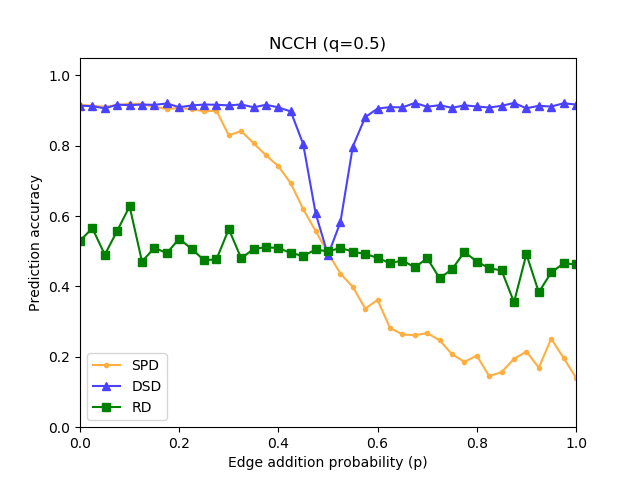
\includegraphics[width=0.7\textwidth]{NCCH_fixq.png}
\caption{Plot showing prediction accuracies of the prediction method using the DSD, SPD, and RD metrics. In this simulation, the parameter $q$ was fixed to $0.5$.}
\label{fig:NCCH_fixq}
\end{figure}

\begin{figure}[H]
\centering
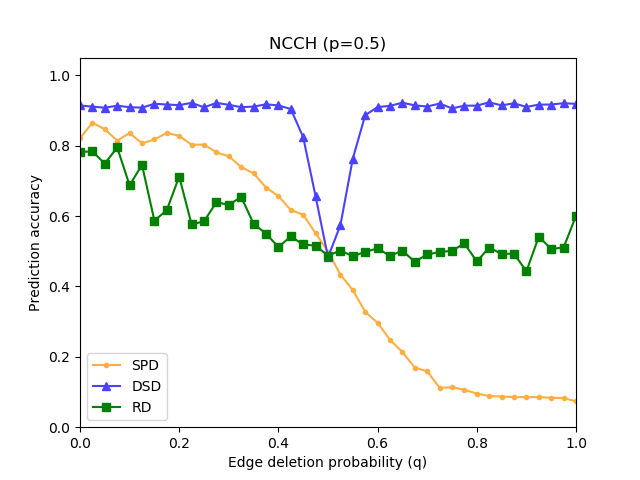
\includegraphics[width=0.7\textwidth]{NCCH_fixp.png}
\caption{Plot showing prediction accuracies of the prediction method using the DSD, SPD, and RD metrics. In this simulation, the parameter $p$ was fixed to $0.5$.}
\label{fig:NCCH_fixp}
\end{figure}

\begin{figure}[H]
\centering
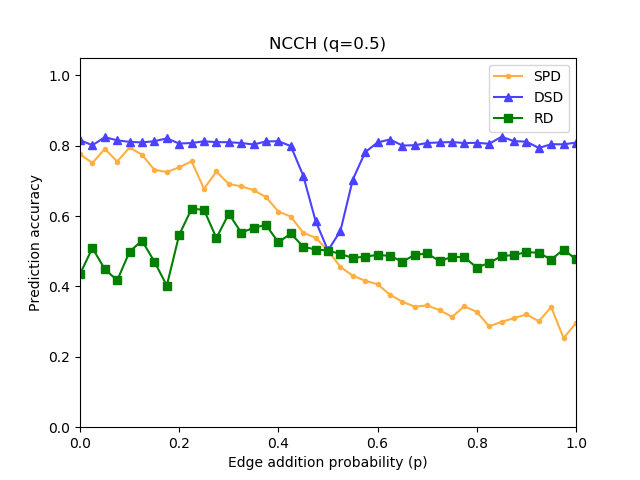
\includegraphics[width=0.8\textwidth]{NCCH_fixq_r300.png}
\caption{Plot showing compressed prediction accuracies for a larger value of the \textit{hubs} parameter. In this simulation, the parameter $q$ was fixed to $0.5$, and \textit{hubs} was set to $300$.}
\label{fig:NCCH_fixq_r300}
\end{figure}

In order to test the effects of the number of hub nodes added, 
prediction accuracies were plotted over the \textit{hubs} parameter. Both 
parameters $p$ and $q$ were set to fixed values such that the prediction
accuracies using DSD, SPD, and RD could be clearly separated. Thus a value
of $p=0.2$ and $q=0.5$ was chosen. These parameters are shown in Table 
\ref{table:NCCH-params-r}.

\begin{table}[H]
\centering
\begin{tabular}{|l|l|}
\hline
$n$ & $250$ \\ \hline
$p$ & $0.2$\\ \hline
$q$ & $0.5$\\ \hline
\textit{hubs} & Range from $0$ to $400$\\ \hline
\textit{hubsP} & $0.8$\\ \hline
$censorP$ & $0.7$\\ \hline
$avgRuns$ & $10$\\ \hline
\end{tabular}
\caption{Tables of parameter values used for our NCCH simulations over the \textit{hubs} parameter.}
\label{table:NCCH-params-r}
\end{table}

\begin{figure}[H]
\centering
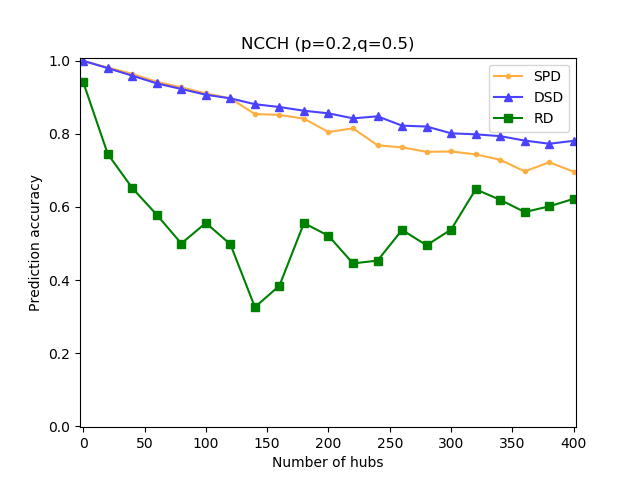
\includegraphics[width=0.8\textwidth]{NCCH_r400.png}
\caption{Plot showing prediction accuracies over the \textit{hubs} parameter. In this simulation, the parameter $p$ was fixed to $0.2$, and $q$ was fixed to $0.5$.}
\label{fig:NCCH_r400}
\end{figure}

\subsection{Analysis}
We can perform a similar analysis to that of the NCC graphs. We can see
in Figures \ref{fig:NCCH_fixq} and \ref{fig:NCCH_fixp} that the shapes of 
the prediction accuracy curves do not change significantly. The main
difference between these plots and the plots for the NCC graphs are that
the plots for NCCH graphs are slightly compressed vertically. This behavior
can be explained by the presence of the hub vertices. Since these hub
vertices are labeled at random, there will always be a proportion of the
vertices in the NCCH graphs that can only be predicted at random. 
Specifically in the case of Figure \ref{fig:NCCH_fixq}, we see that the
prediction accuracies start at $0.9$ rather than $1.0$. If we consider the
number of hub vertices added, $hubs=100$, in relation the the number of
vertices in the NCCH graph, $2n + hubs = 600$, then we can see that since
hub vertices will be predicted at random, we should expect a prediction
accuracy of around $\frac{550}{600} \approx 0.92$. A simulation run with
the parameter $hubs=300$ was run, and shows this idea of compression in
Figure \ref{fig:NCCH_fixq_r300}. The change in the rate of compression can
be seen in Figure \ref{fig:NCCH_r400}.

\section{Class-weighted Barab\'{a}si-Albert (CWBA) Graphs}
In this section, we construct CWBA graphs (Chapter 3) and run label
prediction methods on them. We study the CWBA graphs because they are
scale-free.

\subsection{Data Collection}

\begin{table}[H]
\centering
\begin{subfigure}[h]{0.4\linewidth}
\begin{tabular}{|l|l|}
\hline
$n$ & $1000$ \\ \hline
$m$ & Range from $1$ to $300$\\ \hline
$\rho$ & $2$\\ \hline
$censorP$ & $0.7$\\ \hline
$avgRuns$ & $10$\\ \hline
\end{tabular}
\caption{Fixed $\rho$}
\end{subfigure}
\hfill
\begin{subfigure}[h]{0.4\linewidth}
\begin{tabular}{|l|l|}
\hline
$n$ & $1000$ \\ \hline
$m$ & $300$\\ \hline
$\frac{1}{\rho}$ & Range from $0.05$ to $1$\\ \hline
$censorP$ & $0.7$\\ \hline
$avgRuns$ & $10$\\ \hline
\end{tabular}
\caption{Fixed $\rho$}
\end{subfigure}%
\caption{Tables of parameter values used in our CWBA simulations. The table
on the left shows simulation parameters for a fixed $\rho$, and the table
on the right shows simulation parameters for a fixed $m$ over the inverse of $\rho$.}
\label{table:CWBA-params}
\end{table}

Our CWBA graphs have two input parameters, where $m$ is the minimum vertex
degree, and $\rho$ is the factor of same-class attachment. Table
\ref{table:CWBA-params} shows the parameters used in our simulation. We
also studied the prediction accuracies over $\frac{1}{\rho}$ in order to
study the entire range of values for $\rho$.

\begin{figure}[H]
\centering
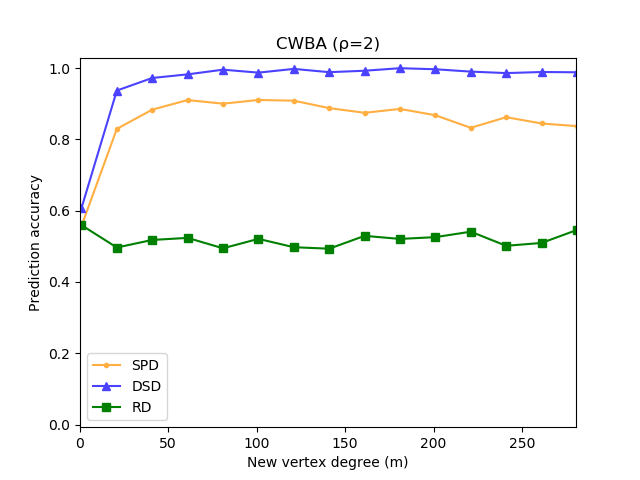
\includegraphics[width=0.8\textwidth]{CWBA_fixrho.png}
\caption{Plot showing prediction accuracies over the $m$ parameter. In this simulation, the parameter $\rho$ was fixed to $2$.}
\label{fig:CWBA_fixrho}
\end{figure}

\begin{figure}[H]
\centering
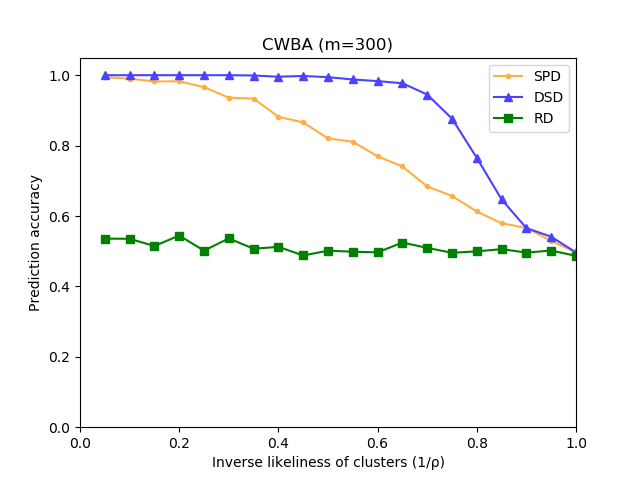
\includegraphics[width=0.8\textwidth]{CWBA_rhoinv.png}
\caption{Plot showing prediction accuracies over the inverse of the $\rho$
parameter. In this simulation, the parameter $m$ was fixed to $300$.}
\label{fig:CWBA_rhoinv}
\end{figure}

\subsection{Analysis}
% Fix when Ch4 done
In our simulations for the CWBA graph, our initial graph is a star $S_m$.
It is important to discuss the extreme cases for CWBA graphs.

\begin{proposition}
When $\rho=1$ for CWBA graphs, we get a randomly labeled scale-free graph.
\end{proposition}
\begin{proof}
We note that when $\rho=1$, the probability of drawing an edge to a vertex $u$ in the CWBA process (Chapter 3) becomes
\[
  p_u = \begin{cases}
    \frac{\deg(u)}{w} &: u \in S_l\\
    
    \frac{\deg(u)}{w} &: u \in (V_G - S_l)\\
  \end{cases}
\]
where
\[
  w = \sum_{v \in S_l}\deg(v) + \sum_{v \in (V_G - S_l)}\deg(v)
\]

We can clearly see that with $\rho=1$, there is no preference in attachment
based on the label, so all vertices are preferentially connected based on
the degree of vertices.
\end{proof}

For $\rho=0$, we can see that vertices with opposite label would only be
considered for attachment, and the opposite would be true for extremely 
high values of $\rho$.

Figures \ref{fig:CWBA_fixrho} and \ref{fig:CWBA_rhoinv} show DSD aids in
predicting more accurately than the other two metrics. Figure 
\ref{fig:CWBA_rhoinv} fixes a value for the parameter $m = 300$ and shows
prediction accuracies over the entire range of values for the $\rho$
parameter. The figure illustrates that when the same-class preferential
attachment factor $\rho$ is $1$, the resulting CWBA graph is random, since
there is no notion of preferential attachment for $\rho=1$. However, for
$\rho > 1$, drawing same-class edges are preferred and this results in a
sharp increase in accuracy for the prediction method using DSD, while the
method using SPD increases at a linear rate. We must note that the 
parameter for minimum vertex degree, $m$, was fixed at $m=300$, so the
resulting CWBA graph is fairly dense. Figure \ref{fig:CWBA_fixrho} shows 
that increasing the parameter $m$ will not change prediction accuracies for
$\rho > 1$, as all of the curves in the plot level out very quickly.

\section{Overall Findings}
After analyzing the results of our simulations, we have found that the 
shortest path distance (SPD) works well with few paths between clusters. The
diffusion state distance (DSD) works well in general as long as neighborhoods
can be distinguished. This can be seen from the NCC and NCCH graph 
simulations. The resistance distance (RD), however, does not seem to work
very well with our simulations, and seems to work best on very sparse graphs.


\chapter{Analysis of Real-World Data}
\label{chap:real_world}
In order to test the conclusions of our experimental results, we also performed analyses on two
real-world data sets. The Coauthor network contains data about statistician coauthorship in
prominent journals, while the email-Eu-Core data set shows email communications within a large
research institution. The data sets were picked based upon their relatively small sizes and easy
interpretability. In both cases, vertices represent humans, which was done in order to test DSD's
performance outside of the biological domain.

Elsewhere, we have used the imprecise term \textbf{hub} to refer to the vertices of unusually high
degree in certain graphs (see page \pageref{def:hubs}). For the purposes of this chapter only, we
will use the following rigorous definition so that we can numerically analyze our data sets.

\begin{definition}
  Let $G$ be a graph. A \textbf{hub} in $G$ is any vertex $v$ whose degree is more than two standard
  deviations above the graph average,

  \[ \deg(v) \geq \mu + 2*\sum_{u \in G}(\deg(u) - \mu^2)^2\]

  where

  \[ \mu = \frac{1}{|G|}\sum_{u \in G}\deg(u) \]
\end{definition}

Under this definition, the number of hubs should be positively correlated with the width of the
degree distribution.


\section{Selected datasets}

\subsection{Coauthor}

The Coauthor data set consist of data collected from four leading statistical journals: The Annals
of Statistics, Biometrika, the Journal of the American Statistical Association, and the Journal of
the Royal Statistical Society. Ji and Jin collected data about all papers published from 2003
through the first half of 2013 and resolved data hygiene issues such as having multiple different
published names for the same author. A graph was then constructed where every vertex corresponded to
a statistician, and edges were inserted to connect any pair of statisticians who had appeared as
coauthors. This graph was then used to cluster the authors into three statistical subdisciplines
using a spectral clustering algorithm, SCORE, which stands for Spectral Clustering On Ratios of
Eigenvalues ~\cite{ji2016}. The labels generated by SCORE showed a high degree of agreement with
other clustering approaches and were found to be reasonable by human researchers, so we believe they
are suitable for use as ground truth labels in a classification experiment. The three labels
identified were ``Objective Bayes,'' ``Biostatistics,'' and ``High-Dimensional Data Analsysis.''

After restricting to the largest connected component, the network has 4388 edges on 2263 vertices,
and so is a relatively sparse graph. The average degree is 3.88, while the max is 65. The number of
hubs is 98, which is $4.43\%$ of all vertices. This graph appears to have a scale-free degree
distribution, as can be seen from Figure \ref{fig:real_world_degree_dist}, and so would be expected
to have a relatively large number of high-degree hubs.

\begin{figure}
  \centering
  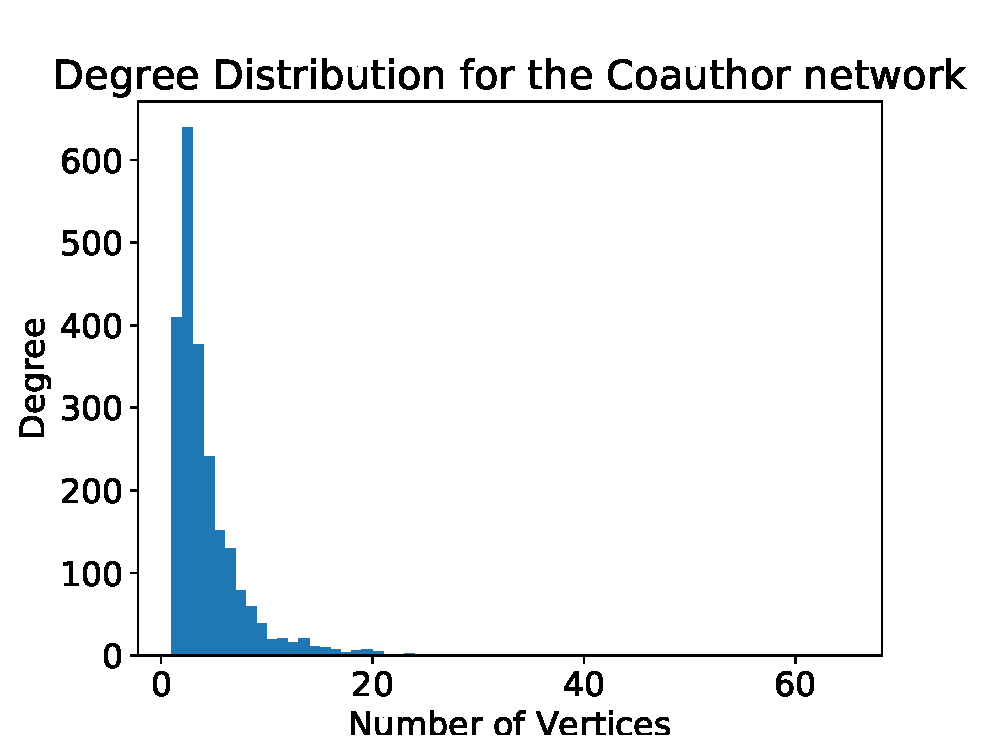
\includegraphics[width=0.48\textwidth]{coauthor_degree_dist.eps}
  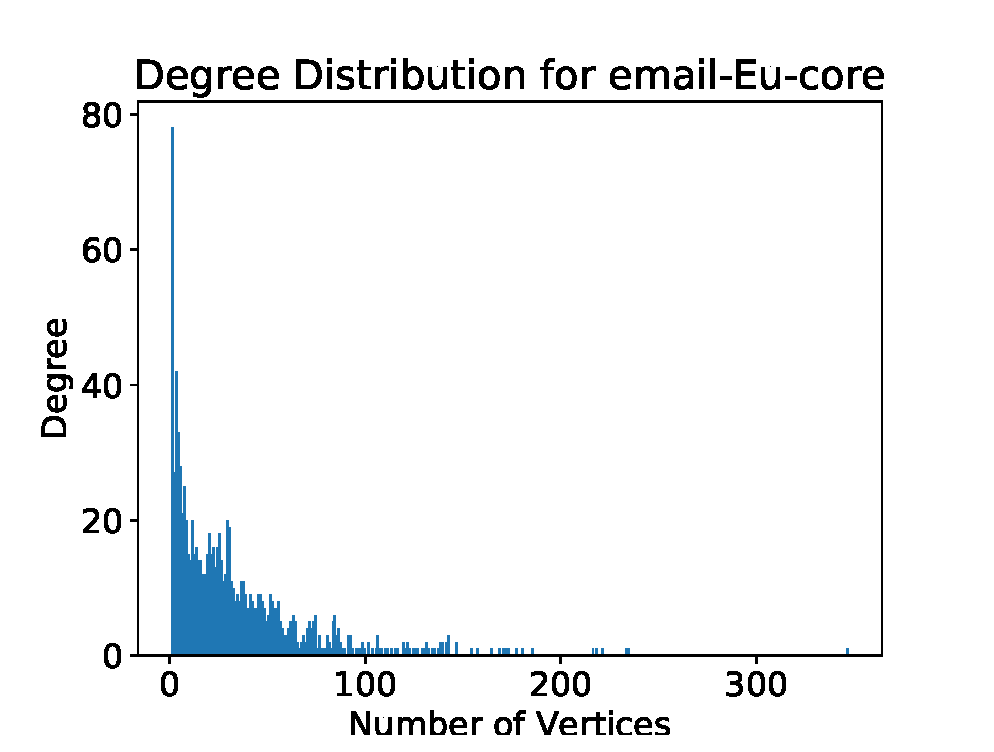
\includegraphics[width=0.48\textwidth]{email_degree_dist.eps}
  \caption{The degree distribution plots for both networks. Both plots appear to show scale-free
    distributions.}
  \label{fig:real_world_degree_dist}
\end{figure}


\subsection{email-Eu-core}

The email-Eu-core data set is built from email data collected over the course of 18 months from 2003
to 2005 at a European research institution. Each vertex corresponds to an employee at the
institution, and is labeled an integer indicating that person's department. There are a total of 48
departments in the data set. An edge was drawn between any two parties which exchanged an email over
the time period in question ~\cite{snapnets}. The original version of this data set was directed,
but we discard edge direction information for our analysis.

This graph has 986 vertices and 25571 edges after reducing to the largest connected component. The
average degree of the graph is 33.9, with the maximum being 347. The number of hubs is 49, which is
$4.97\%$ of the entire graph-- strikingly similar to the Coauthor network. Also, compared to the
Coauthor network, this graph is somewhat smaller and substantially denser, which makes it an
attractive candidate for demonstrating the efficacy of DSD, as such a graph would be expected to
have more and higher degree hubs than a less dense one.

In addition and in spite of its small size, this graph has 48 possible labels, indicating an average
class size of just $20.54$ elements. This means that we also have to be more conservative in
censoring data on this graph, as it would be easy to censor too high a proportion of one of the
smaller classes to be able to accurately recover the labels.


\section{Results and Analysis}

In order to evaluate the efficacy of each classifier, the label prediction experiment was done using
5-fold cross-validation on each predictor. Cross-validation is a common machine learning technique
where the point set (in our case, the vertex set of the graph) is divided into $k$ equal-size
\textbf{folds}. Each fold is censored one at a time, and a trial is run using a predictor built from
the uncensored data. These trial accuracies are then averaged in order to compute an overall
measurement of accuracy. The primary advantage of cross validation is that it forces prediction to
be run on every single vertex of the graph. A disadvantage is that it requires use of small
censorship proportions. In this case, $20\%$ of vertices would be censored in each run.

$k=20$ was used as the parameter for the nearest neighbors algorithm. The results are summarized in
the bar plot in Figure \ref{fig:real_world_results}.

\begin{figure}[H]
  \centering
  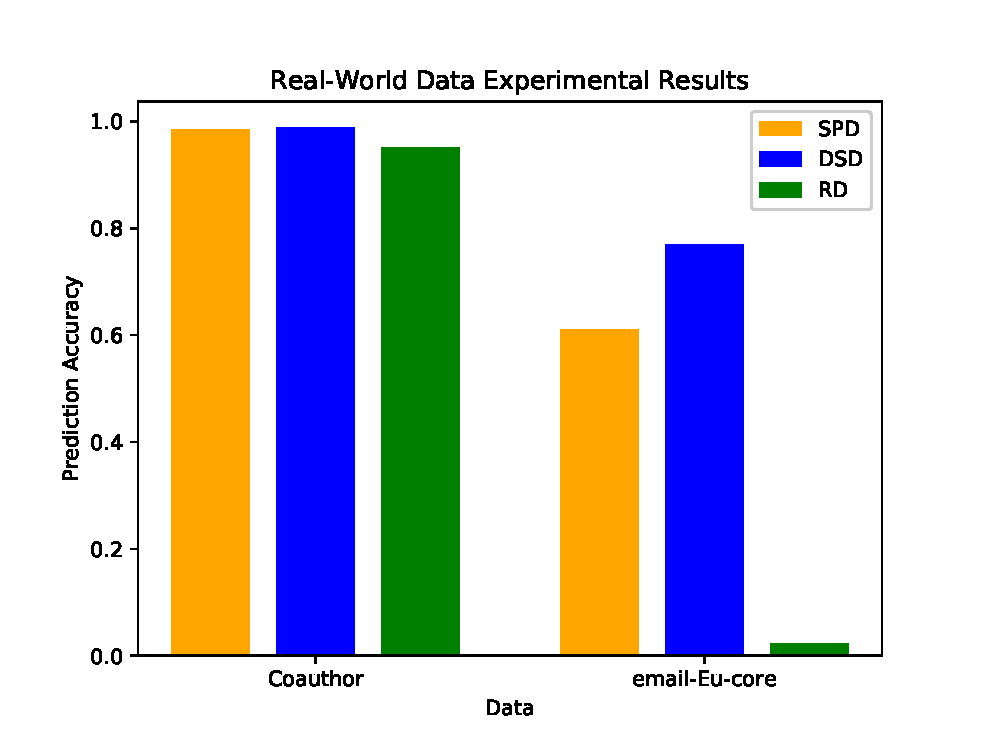
\includegraphics[width=\textwidth]{real_world_results.eps}
  \caption{Real-world data prediction accuracy results.}
  \label{fig:real_world_results}
\end{figure}

The Coauthor results are especially striking, as all three metrics, including resistance distance,
performed extremely well. This could probably be explained, at least partially, by the fact that the
Coauthor network is fairly sparse and that the number of labels is small. The lower censorship
proportion, $20\%$ as compared to the $70\%$ used in the simulated experiments, probably contributes
to the high accuracies as well, but informal experiments using random censoring at high proportions
yield very similar results.

It seems likely that the high label prediction performance is mostly due to the fact that SCORE was
used to generate ground truth. For some reason, the SCORE communities are clustered extremely
tightly irrespective of the metric. This is an interesting finding in its own right because it
suggests that the way that we think about clusters, at least in the context spectral clustering,
probably doesn't capture some important properties of the communities found in real-world data. The
fact that resistance distance works well on the spectral clusters but not the real ground truth is
especially noteworthy in this regard.

By contrast, the email-Eu-core results are much less surprising. DSD clearly provides the dominant
classification algorithm, followed by a surprisingly strong showing from SPD. RD performs like
random guesses, as it did with most of the simulated data (recall that as there are 48 classes,
uniform random guessing would yield an expected success rate of $1/48$, or about $2.1\%$).

These results suggest that DSD has some sort of built-in model of community structure which agrees
with the real-world data. We expect that these results would generalize to work well with a wide
variety of network structures, but particularly those whose topology represents some sort of
information exchange.


%%% Local Variables:
%%% mode: latex
%%% TeX-master: "../Main"
%%% End:



\chapter{Conclusions}
\label{chap:conclusions}
Our project hopes to provide information about what makes prediction methods using the diffusion
state distance (DSD) metric work better than methods using other metrics on graphs. Our simulation
models were constructed to attempt to identify structures within graphs that caused the DSD to work
better. In Chapter 3, we proposed the novel Noisy Complete Components (NCC) and Noisy Complete
Components with Hubs (NCCH) models in order to see whether tightly clustered graphs and dense
neighborhoods would affect prediction using the DSD. We also developed the Class-Weighted
Barab\'{a}si-Albert (CWBA) model in order to see the effects of scale-free properties on prediction
using the DSD.

Using our simulation models, we experimented with various parameters of our models in order to get data about changes in prediction accuracy with respect to changes in the graph structure (Chapter 6). We tested parameters that affected neighborhoods of vertices in our models as well as the number of hub vertices. More models could be constructed in future work to draw out characteristics of graph structure that the DSD metric is most affected by. Also, subject-knowledge for specific types of networks, mentioned in Chapter 5, could be added to the models to add to our metric-based clustering algorithm.

Our simulation results show that the DSD is more effective at detecting some 
properties of graph structure than the shortest path distance and the
resistance distance for dense graphs. Prediction methods using the DSD were 
shown to be more robust to hub vertices and our NCC simulations were able to
intuitively show how the DSD determines communities based on neighborhoods 
rather than direct neighbors. Our project could have included simulations to
study the resistance distance metric as well, and graph models that would
cause the DSD metric to cause prediction accuracies to be significantly 
worse than the shortest path distance.

Our analysis of real-world networks (coauthor, email-Eu-core) did not provide
as much information as we expected on how the DSD metric is useful on examples
of real networks. However, both still showed that the DSD metric performed
best of the three metrics that we studied.

There are many interesting questions remaining. For what parameters for CWBA graphs would the SPD perform better than the DSD? We believe that such 
an investigation would provide further insight into properties of scale-free networks which would indicate the most appropriate metric for classification
problems on scale-free networks. This analysis could also examine other 
statistics on graphs such as betweenness centrality~\cite{newman2005measure} and eigencentrality based on dissimilarity measures~\cite{alvarez2015eigencentrality}
to see whether they are correlated with DSD performance. The effectiveness of the DSD in detecting manifold-like structures of
graphs is also a challenge that could be explored. Several simulation models could be
constructed to study this question. Also, the effect of the DSD metric in
detecting the dispersion of rumors or the spread of information could also
be studied. This would relate to the virality of news, products, clothing, and other trends. The way the DSD metric is defined by random walks seems to give
a hint for what kinds of real-world data that it should be experimented with.
The DSD metric could be compared to heat dispersion and different kinds
of dispersions in nature, such as the dispersion of particles or biological
dispersion of pollen and seeds. Such studies could provide a more accurate
understanding of how natural biological networks interact with each other.


\bibliography{biblio}
\bibliographystyle{plain}

\end{document}
